\chapter{MAGIC4FDG系统的详细设计与实现}

第三章完成了需求分析和概要设计，本章在此基础上对核心模块进行详细设计和实现展示。本章将逐一剖析知识提取模块、策略规划与代码生成模块、模糊测试与覆盖率收集模块、缺口诊断模块的内部结构和实现机制。每节先用类图和顺序图说明设计思路，再结合关键代码片段展示核心功能的具体实现。

\section{知识提取模块详细设计与实现}

知识提取模块是整个系统的基础，没有它提供的结构化API知识，后面的智能体就无从下手。它的职责是在Docker容器内编译目标库并做clang AST导出，从中提取结构化的API知识，再根据不同智能体的需求把知识格式化为适合注入提示词的文本片段。下面先通过类图和顺序图说明设计思路，再深入解析AST解析与知识构建、差异化上下文构建两个核心功能的实现。

\subsection{知识提取模块详细设计}

图\ref{fig:knowledge-class}是知识提取模块的详细设计类图，展示了关键类及其属性和方法。


模块入口为\texttt{extract\_knowledge}函数，接收目标库配置后依次执行AST解析、宏提取、调用图构建、语义标注、注释附加五个阶段，最终产出\texttt{KnowledgeStore}对象。\texttt{KnowledgeStore}在设计上充当全局知识容器，内含四个字段。其中\texttt{api\_entries}存放全部公开API条目，每条对应一个\texttt{APIEntry}实例，记录函数名、签名、返回类型、参数列表等基本信息，同时包含功能类别、前置条件和文档注释。\texttt{call\_graph}用邻接表存储函数间的调用关系。其余两个字段分别管理类型定义（结构体、枚举、类型别名）和宏常量，宏常量还按标志位、普通常量、函数式宏做了分类，方便后续生成智能体按需取用。

\begin{figure}[H]
    \centering
    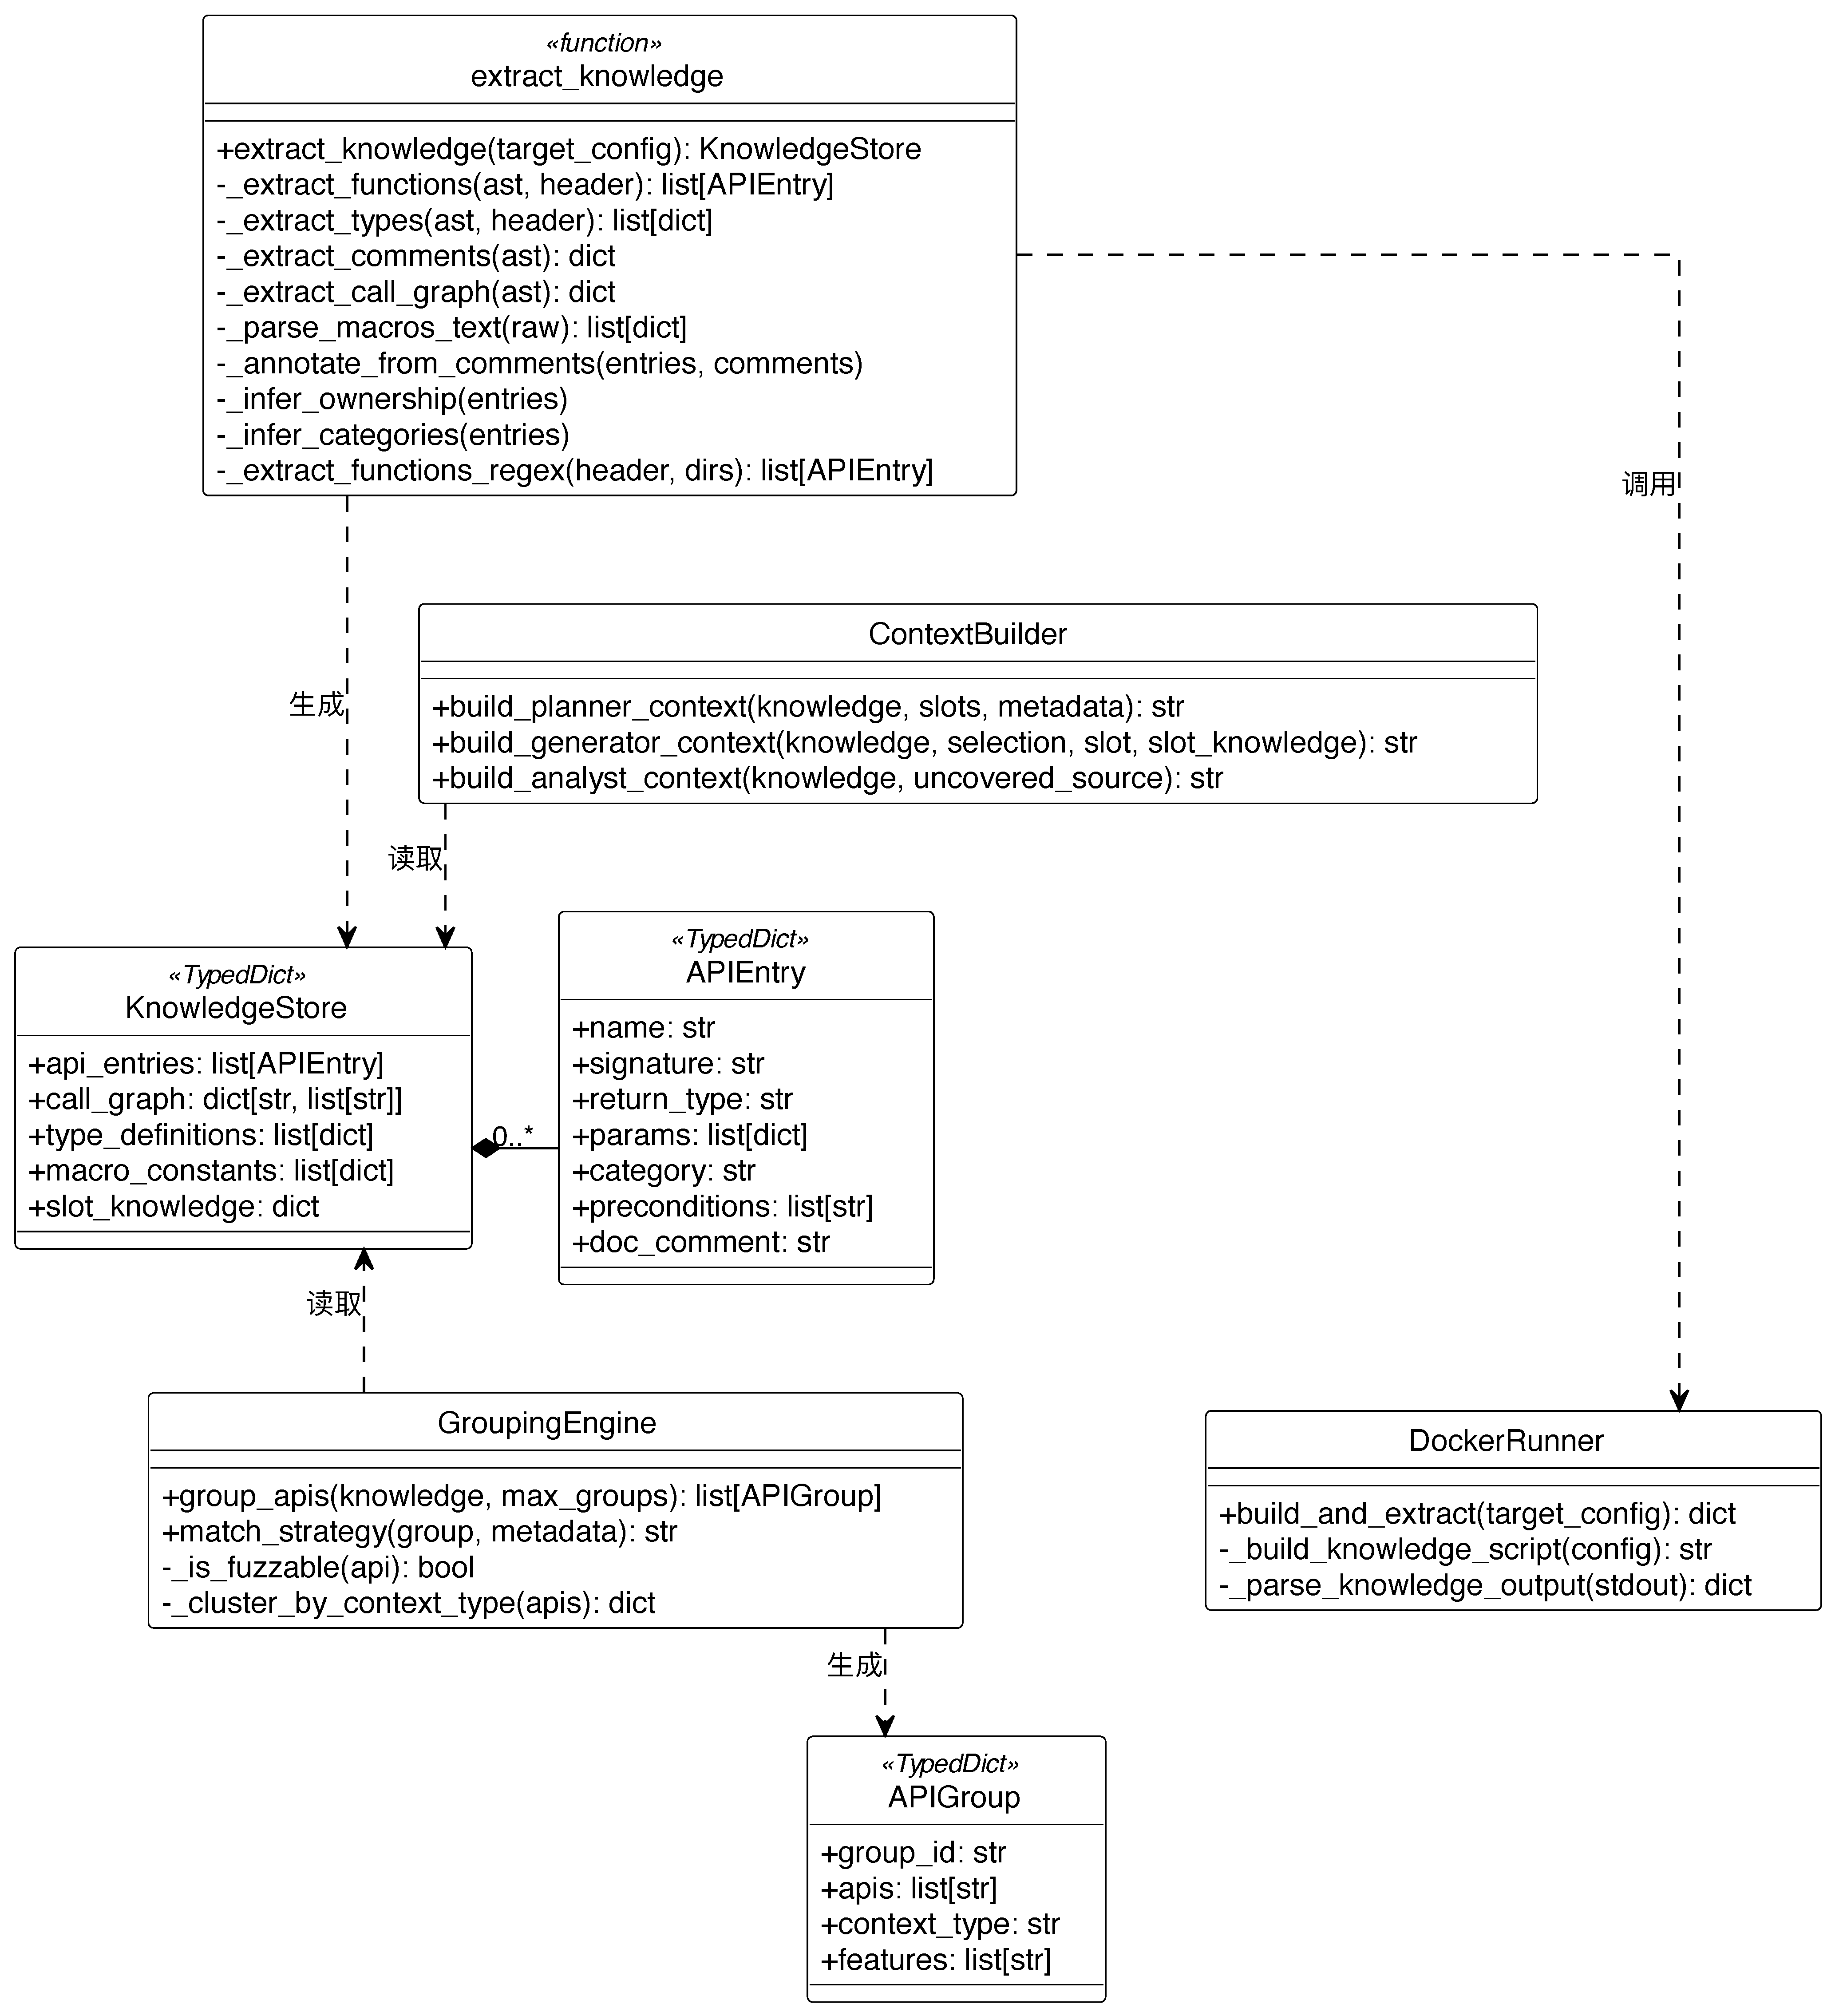
\includegraphics[width=\textwidth]{images/knowledge_class.pdf}
    \caption{知识提取模块详细设计类图}
    \label{fig:knowledge-class}
\end{figure}

\texttt{ContextBuilder}类是知识处理的核心组件，负责把原始\texttt{KnowledgeStore}转换为适合注入提示词的文本片段。它提供三个方法：\texttt{build\_planner\_context}为Planner生成API分类概览和调用图摘要；\texttt{build\_generator\_context}为Generation生成目标API完整签名、参数语义和类型定义的详细上下文；\texttt{build\_analyst\_context}为Analyst生成完整API清单和未覆盖源码行的诊断上下文。三种上下文的信息粒度和侧重点各不相同，这就是差异化上下文注入的体现。

\texttt{GroupingEngine}类实现确定性的API分组和策略匹配，作为LLM策略规划失败时的回退方案。\texttt{group\_apis}方法基于调用图连通分量和参数类型相似性做API聚类，\texttt{match\_strategy}方法用规则引擎把分组特征与策略元数据的适用条件匹配。

\begin{figure}[H]
    \centering
    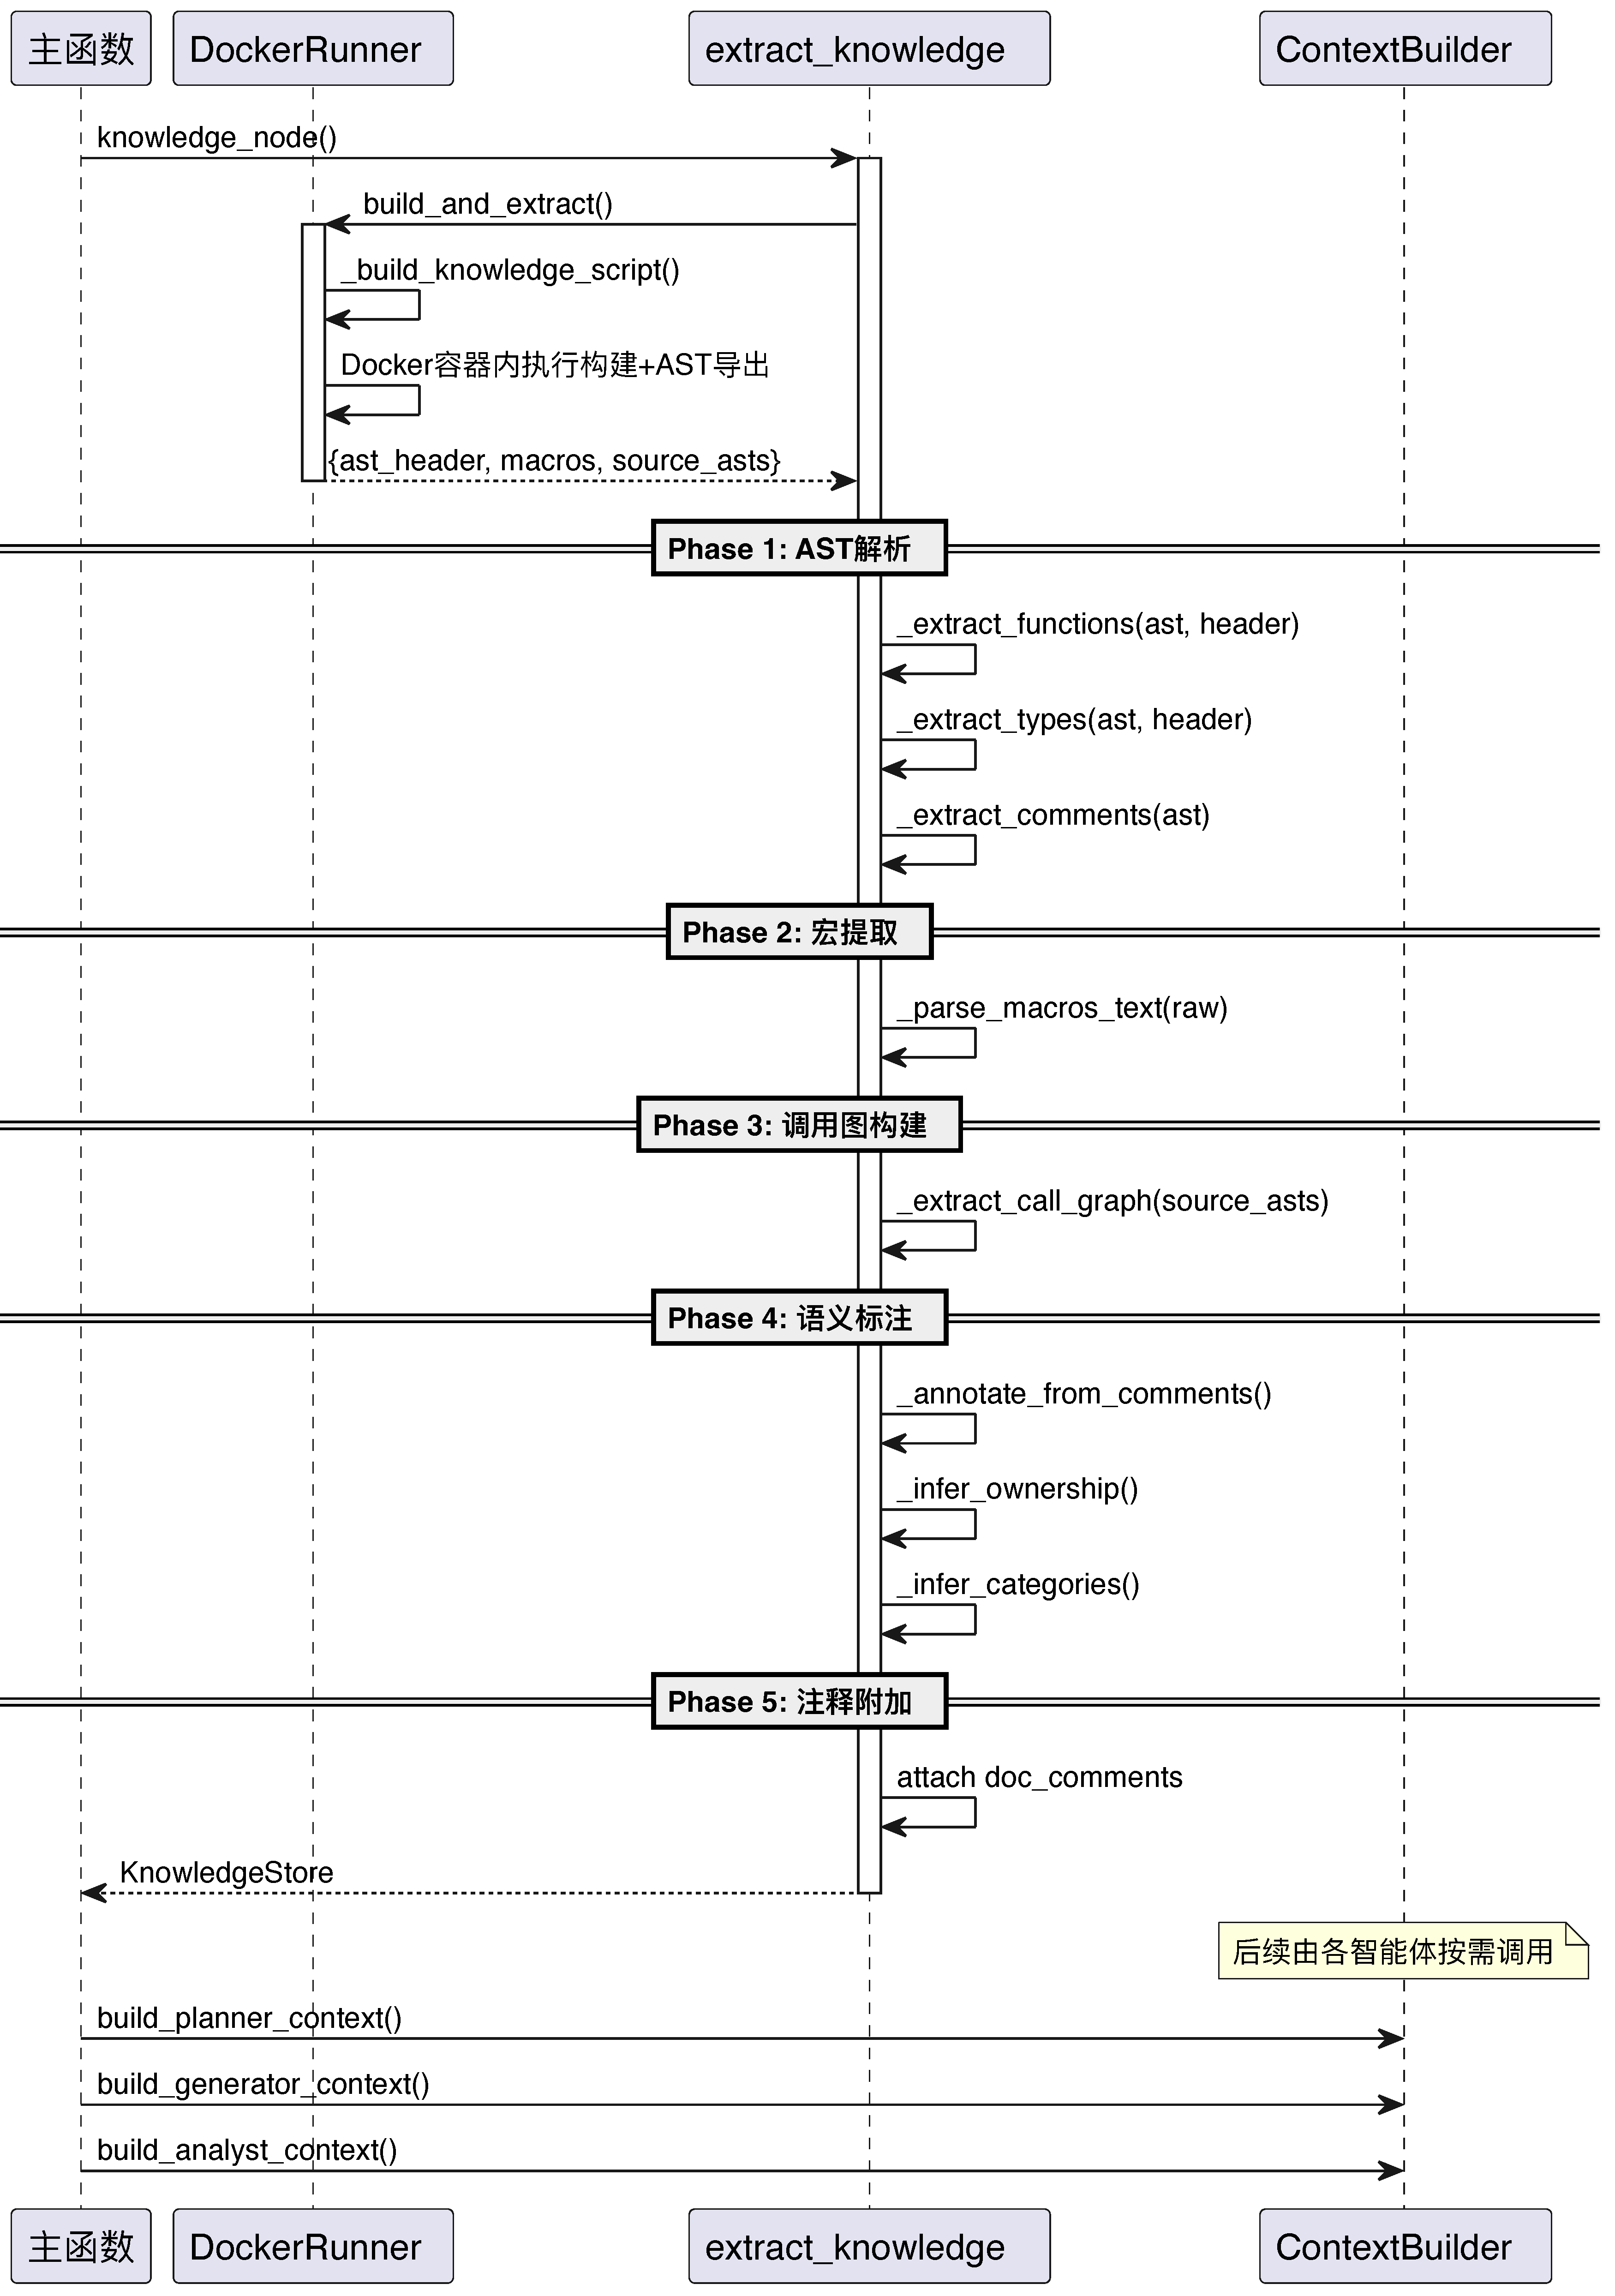
\includegraphics[width=\textwidth]{images/knowledge_seq.pdf}
    \caption{知识提取模块详细设计顺序图}
    \label{fig:knowledge-seq}
\end{figure}

图\ref{fig:knowledge-seq}是知识提取模块的顺序图，描绘了各功能类之间的协作时序。

流程从主函数调用\texttt{knowledge\_node}开始。该函数读取流水线状态中的目标库配置，随即委托\texttt{extract\_knowledge}完成实际工作。后者首先通过\texttt{DockerRunner}的\texttt{build\_and\_extract}方法，在Docker容器内完成四项操作：目标库编译、头文件AST导出、预处理器宏导出、源文件AST导出。容器执行结果经标准输出的分隔符协议传回宿主机。

获取原始数据后进入五阶段处理流水线：第一阶段调用\texttt{\_extract\_functions}解析头文件AST JSON，遍历\texttt{FunctionDecl}节点提取公开API签名；第二阶段调用\texttt{\_parse\_macros\_text}解析预处理器输出，提取并分类宏常量；第三阶段对每个源文件AST调用\texttt{\_extract\_call\_graph}，该步骤的核心逻辑在于递归查找\texttt{CallExpr}节点、将调用关系填入邻接表。第四阶段较为复杂，需要连续执行三个语义标注方法：\texttt{\_annotate\_from\_comments}、\texttt{\_infer\_ownership}、\texttt{\_infer\_categories}，从注释和命名规则中推断所有权语义、前置条件和功能类别。第五阶段将文档注释附加到对应API条目。如果AST解析阶段未能提取到任何函数声明，系统自动回退到基于正则表达式的头文件扫描方案，保证知识提取不会完全失败。


\subsection{AST解析与知识构建功能实现}

这一小节聚焦知识提取模块中AST解析与知识构建的实现细节。本节依次说明clang AST深度优先遍历算法、函数签名提取、调用图构建和语义标注这四个功能的具体做法。

\subsubsection{AST深度优先遍历}

clang以JSON格式导出的抽象语法树本质上是一棵嵌套树，每个节点通过\texttt{inner}字段持有子节点列表。本模块实现了一个通用的深度优先遍历生成器\texttt{\_walk\_ast}，它是后续所有AST分析功能的基础。这里有一个实现细节：生成器采用Python的\texttt{yield from}语法做惰性遍历，不会一次性把整棵AST展开到内存里。对于大型库（如OpenSSL，AST JSON可达数百MB），这一点至关重要。该遍历器的实现如图\ref{fig:walk-ast}所示。

\begin{figure}[H]
    \centering
    \begin{lstlisting}[style=style@python]
   def _walk_ast(node: dict):
       if not node:
           return
       yield node
       for child in node.get("inner", []):
           if child:
               yield from _walk_ast(child)
    \end{lstlisting}
    \caption{AST深度优先遍历生成器}
    \label{fig:walk-ast}
\end{figure}

\subsubsection{函数签名提取}

函数签名提取是知识构建中最关键的一步，目标在于从AST中定位所有公开API的函数声明，并提取函数名、完整类型签名、返回类型及参数列表。核心实现如图\ref{fig:extract-functions}所示。

实现中采用了逐层收窄的过滤策略。首先，通过\texttt{kind}字段筛出\texttt{FunctionDecl}节点，排除变量声明和类型定义。接着检查\texttt{loc}字段中的文件路径，只有声明在目标头文件中的函数才予以保留，系统头文件和第三方依赖引入的声明在此被剔除。最后一道过滤针对函数名前缀：以下划线开头的内部实现函数不进入结果集。通过这三道过滤的函数声明，系统从\texttt{type.qualType}字段取出完整函数类型签名，并调用\texttt{\_extract\_params}方法遍历子节点中的\texttt{ParmVarDecl}节点，逐一提取参数名、类型、是否可空和所有权语义。

当AST解析未能提取到任何函数声明时（比如目标库使用了clang无法处理的非标准扩展），系统会自动回退到基于正则表达式的头文件扫描方案。这个回退方案用多行正则匹配C函数声明的标准模式。精度虽然不如AST解析，但能保证知识提取流程不会因为单一工具链的局限而彻底失败。

\begin{figure}[H]
    \centering
    \begin{lstlisting}[style=style@python]
   def _extract_functions(ast: dict, header_path: str) -> list[APIEntry]:
       entries: list[APIEntry] = []
       header_name = Path(header_path).name if header_path else ""
       for node in _walk_ast(ast):
           if node.get("kind") != "FunctionDecl":
               continue
           loc = node.get("loc", {})
           file_field = (loc.get("file", "") or
                         loc.get("expansionLoc", {}).get("file", ""))
           if file_field and header_name and header_name not in file_field:
               continue
           name = node.get("name", "")
           if not name or name.startswith("_"):
               continue
           qual_type = node.get("type", {}).get("qualType", "")
           params = _extract_params(node)
           return_type = _infer_return_type(qual_type)
           entries.append(APIEntry(
               name=name, signature=qual_type,
               return_type=return_type, params=params,
               category="utility", preconditions=[],
               group="", doc_comment="",
           ))
       return entries
    \end{lstlisting}
    \caption{基于AST的函数签名提取}
    \label{fig:extract-functions}
\end{figure}

\subsubsection{调用图构建}

调用图记录了函数之间的调用关系，是策略规划智能体做API分组和场景设计时的重要依据。系统通过递归遍历源文件AST中的\texttt{CallExpr}节点来构建调用图，核心实现如图\ref{fig:call-graph}所示。

算法维护一个\texttt{current\_func}状态变量，遍历过程中持续跟踪当前所处的函数作用域。遇到\texttt{FunctionDecl}节点时更新当前函数名；遇到\texttt{CallExpr}节点时通过\texttt{\_resolve\_callee}解析被调用函数的名称，把调用关系记录到邻接表中。值得说明的是，\texttt{\_resolve\_callee}方法需要处理两种常见的AST表示：直接的\texttt{DeclRefExpr}引用，以及经过\texttt{ImplicitCastExpr}隐式转换的间接引用。系统对所有源文件的调用图做合并和去重，最终生成全局的函数调用关系图。

\begin{figure}[H]
    \centering
    \begin{lstlisting}[style=style@python]
   def _extract_calls_recursive(node: dict, current_func: str,
                                graph: dict) -> None:
       kind = node.get("kind", "")
       if kind == "FunctionDecl":
           current_func = node.get("name", "")
       elif kind == "CallExpr" and current_func:
           for child in node.get("inner", []):
               callee = _resolve_callee(child)
               if callee:
                   graph.setdefault(current_func, []).append(callee)
                   break
       for child in node.get("inner", []):
           if child:
               _extract_calls_recursive(child, current_func, graph)
    \end{lstlisting}
    \caption{调用图递归构建}
    \label{fig:call-graph}
\end{figure}

\subsubsection{语义标注}

语义标注阶段要解决的问题是，光有函数签名还不够，代码生成智能体需要知道如何正确调用这些API。因此本模块从文档注释和函数命名规则两个渠道推断所有权语义、前置条件和功能类别。具体分为三个独立的标注方法。

\texttt{\_annotate\_from\_comments}方法的思路比较直接，用预定义的正则模式集扫描文档注释。系统预定义了三类正则模式集。一类匹配返回值所有权描述，如"caller is responsible to free"；一类匹配参数所有权转移，如"takes ownership"；还有一类匹配前置条件，如"must not be NULL"。注释文本一旦命中某个模式，对应API条目即被打上相应标记。这种模式匹配方案精度有限，但对文档规范的库而言效果尚可。

\texttt{\_infer\_ownership}方法走的是另一条路径——从函数名本身推断语义。具体而言，名字中包含Create、New、Alloc等关键词的函数，其返回值被标记为调用者负责释放；名字中包含Delete、Free、Destroy的函数，其指针参数被标记为所有权转移。实现如图\ref{fig:infer-ownership}所示。

\texttt{\_infer\_categories}方法把每个API归入六个功能类别：解析、创建、销毁、修改、查询、序列化。分类逻辑是按优先级匹配函数名中的关键词，首个命中的类别就是最终结果。这个分类信息后面策略规划智能体会用到，举个例子，系统会把解析类和序列化类API配对来构建往返测试场景。

\begin{figure}[H]
    \centering
    \begin{lstlisting}[style=style@python]
   def _infer_ownership(entries: list[APIEntry]) -> None:
       create_pattern = re.compile(
           r"(Create|New|Duplicate|Copy|Clone|Alloc)", re.I)
       delete_pattern = re.compile(
           r"(Delete|Free|Destroy|Release|Close)", re.I)
       for entry in entries:
           name = entry["name"]
           if create_pattern.search(name) and "*" in entry["return_type"]:
               precond = "Return value must be freed by caller"
               if precond not in entry["preconditions"]:
                   entry["preconditions"].append(precond)
           if delete_pattern.search(name):
               for p in entry["params"]:
                   if "*" in p["type"] and p["ownership"] == "borrow":
                       p["ownership"] = "transfer"
                       break
    \end{lstlisting}
    \caption{基于命名规则的所有权推断}
    \label{fig:infer-ownership}
\end{figure}

\subsection{差异化上下文构建功能实现}

本小节解析\texttt{ContextBuilder}模块的实现。它在\texttt{KnowledgeStore}和大语言模型提示词之间起到翻译作用，针对不同智能体的任务特点，从完整知识库中筛选相关子集并格式化为结构化Markdown文本。本模块提供三种差异化上下文视图。背后的设计原则可以概括为信息不对称：让每个智能体只看到完成任务所需的最小充分信息集，避免无关内容干扰大语言模型推理。

\subsubsection{策略规划上下文}

\texttt{build\_planner\_context}方法为策略规划智能体构建宏观视角的知识上下文。核心思路是提供"广度优先"的信息，让规划智能体了解目标库的整体API分布和函数间关系，而不是单个API的实现细节。实现如图\ref{fig:planner-context}所示。

输出的上下文分为四个信息层次。第一层是按功能类别分组的API概览，展示每个类别的函数数量和签名摘要，帮助规划智能体把握库的功能分布。第二层是调用图摘要，只展示公开API之间的调用关系（内部实现函数被过滤掉），帮助识别API间的依赖链。第三层是关键类型定义摘要，展示结构体字段和枚举值。第四层是当前各槽位的状态信息（仅在第二轮及之后包含），展示每个槽位的策略历史和覆盖率变化趋势，供规划智能体做决策。

\begin{figure}[H]
    \centering
    \begin{lstlisting}[style=style@python]
   def build_planner_context(knowledge: KnowledgeStore,
                                  slots: list[HarnessSlot],
                                  strategy_metadata: list[dict]) -> str:
       lines = ["## Target Library API Surface\n"]
       by_category: dict[str, list] = {}
       for api in knowledge["api_entries"]:
           by_category.setdefault(api["category"], []).append(api)
       for cat in ["parse", "create", "modify", "query",
                   "delete", "serialize", "utility"]:
           apis = by_category.get(cat, [])
           if apis:
               lines.append(f"### {cat.title()} ({len(apis)} functions)\n")
               for api in apis:
                   params_str = ", ".join(
                       f"{p['type']} {p['name']}" for p in api.get("params", []))
                   lines.append(
                       f"- `{api['return_type']} {api['name']}({params_str})`")
       # ... 调用图 + 类型定义 + slot状态
       return "\n".join(lines)
    \end{lstlisting}
    \caption{策略规划上下文构建}
    \label{fig:planner-context}
\end{figure}

\subsubsection{代码生成上下文}

\texttt{build\_generator\_context}方法为代码生成智能体构建"深度优先"的详细上下文。与规划上下文的宏观视角不同，生成上下文聚焦于规划智能体指定的目标API子集，提供生成正确模糊驱动代码所需的全部细节。核心实现如图\ref{fig:generator-context}所示。

\begin{figure}[H]
    \centering
    \begin{lstlisting}[style=style@python]
   def build_generator_context(knowledge: KnowledgeStore,
                                    selection: StrategySelection,
                                    slot: HarnessSlot | None = None,
                                    slot_knowledge: dict | None = None) -> str:
       lines = ["## API Knowledge\n"]
       target_api_names = set(selection.get("target_apis", []))
       relevant_apis = list(knowledge["api_entries"])
       if target_api_names:
           relevant_apis = [a for a in knowledge["api_entries"]
                            if a["name"] in target_api_names]
           for api_name in list(target_api_names):
               callees = knowledge["call_graph"].get(api_name, [])
               for callee in callees:
                   for a in knowledge["api_entries"]:
                       if a["name"] == callee and a not in relevant_apis:
                           relevant_apis.append(a)
       # ... 详细API信息 + 类型定义 + 宏常量 + 累积约束
       return "\n".join(lines)
    \end{lstlisting}
    \caption{代码生成上下文构建}
    \label{fig:generator-context}
\end{figure}

这步的关键在于三个设计决策。第一，API范围做了聚焦：如果规划智能体指定了\texttt{target\_apis}，生成上下文就只包含目标API和它们在调用图中直接调用的函数，其余一概不提供。此处的设计考虑是，无关API信息会稀释大语言模型的注意力，少即是多。第二，信息排序做了优化：同一功能类别内，有文档注释的API排前面，让模型优先看到信息最丰富的接口。第三，跨轮次知识会注入进来：从该槽位隔离的\texttt{SlotKnowledge}中取出累积的约束、正向模式和负向模式一并注入，使大语言模型能利用历史经验，避免反复触发同一类错误。

\subsubsection{缺口诊断上下文}

\texttt{build\_analyst\_context}方法为缺口诊断智能体构建以覆盖率缺口为中心的诊断上下文。设计目标是提供诊断覆盖率问题所需的完整信息链，从未覆盖的源码行出发，结合API清单和调用图，帮助诊断智能体推断覆盖率缺口的根因。核心实现如图\ref{fig:analyst-context}所示。

\begin{figure}[H]
    \centering
    \begin{lstlisting}[style=style@python]
   def build_analyst_context(knowledge: KnowledgeStore,
                                  uncovered_source: dict | None = None) -> str:
       lines = ["## Full API Inventory\n"]
       for api in knowledge["api_entries"]:
           ownership_mark = ""
           if any(p.get("ownership") == "transfer"
                  for p in api.get("params", [])):
               ownership_mark = " [takes ownership]"
           lines.append(
               f"- `{api['signature']}` [{api['category']}]{ownership_mark}")
       # 调用图 + 宏常量标志 + 未覆盖源码行
       if uncovered_source:
           lines.append("## Uncovered Source Lines\n")
           for filename, line_map in list(uncovered_source.items())[:5]:
               lines.append(f"### {filename}")
               for line_no, code in sorted(line_map.items())[:20]:
                   lines.append(f"  {line_no}: {code.rstrip()}")
       return "\n".join(lines)
    \end{lstlisting}
    \caption{缺口诊断上下文构建}
    \label{fig:analyst-context}
\end{figure}

与前两种上下文不同，诊断上下文传递完整的API清单而非子集。原因在于诊断智能体需要判断哪些API尚未被任何驱动覆盖。另一个特点是，该上下文包含未覆盖源码行的原始文本（每个文件最多展示20行），让诊断智能体能直接观察未覆盖代码的具体逻辑，从而给出精确的改进建议。调用图信息则帮助诊断智能体理解函数间的依赖关系，比如某个函数未被覆盖，可能是因为其前置调用函数未被正确初始化。

表\ref{tab:context-comparison}总结了三种上下文视图的信息差异。

\begin{table}[H]
    \centering
    \caption{三种差异化上下文视图的信息对比}
    \label{tab:context-comparison}
    \begin{tabular}{lccc}
        \toprule
        信息维度 & 规划上下文 & 生成上下文 & 诊断上下文 \\
        \midrule
        API范围 & 全量（按类别分组） & 目标子集（含被调用者） & 全量（含所有权标记） \\
        参数详情 & 类型摘要 & 完整（含ownership） & 无 \\
        调用图 & 公开API间关系 & 无 & 完整调用图 \\
        类型定义 & 摘要 & 完整（含字段） & 无 \\
        宏常量 & 无 & 完整（分类展示） & 仅标志位 \\
        覆盖率信息 & 槽位历史趋势 & 无 & 未覆盖源码行 \\
        累积知识 & 无 & 约束+正/负模式 & 无 \\
        \bottomrule
    \end{tabular}
\end{table}

\section{策略规划与代码生成模块详细设计与实现}

策略规划与代码生成模块是整个MAGIC4FDG系统中对大语言模型能力要求最高的部分。其核心任务是将前面提取出来的结构化API知识转化为能编译、能运行的模糊驱动代码。内部由两个智能体协作完成：规划智能体利用大语言模型的语义推理来设计测试场景、分配策略；生成智能体根据规划结果和策略库的指导调用大语言模型编写具体代码。本节先用类图和顺序图阐明模块设计，再分别展开探索阶段策略规划和多提示词策略驱动生成的实现。

\begin{figure}[H]
    \centering
    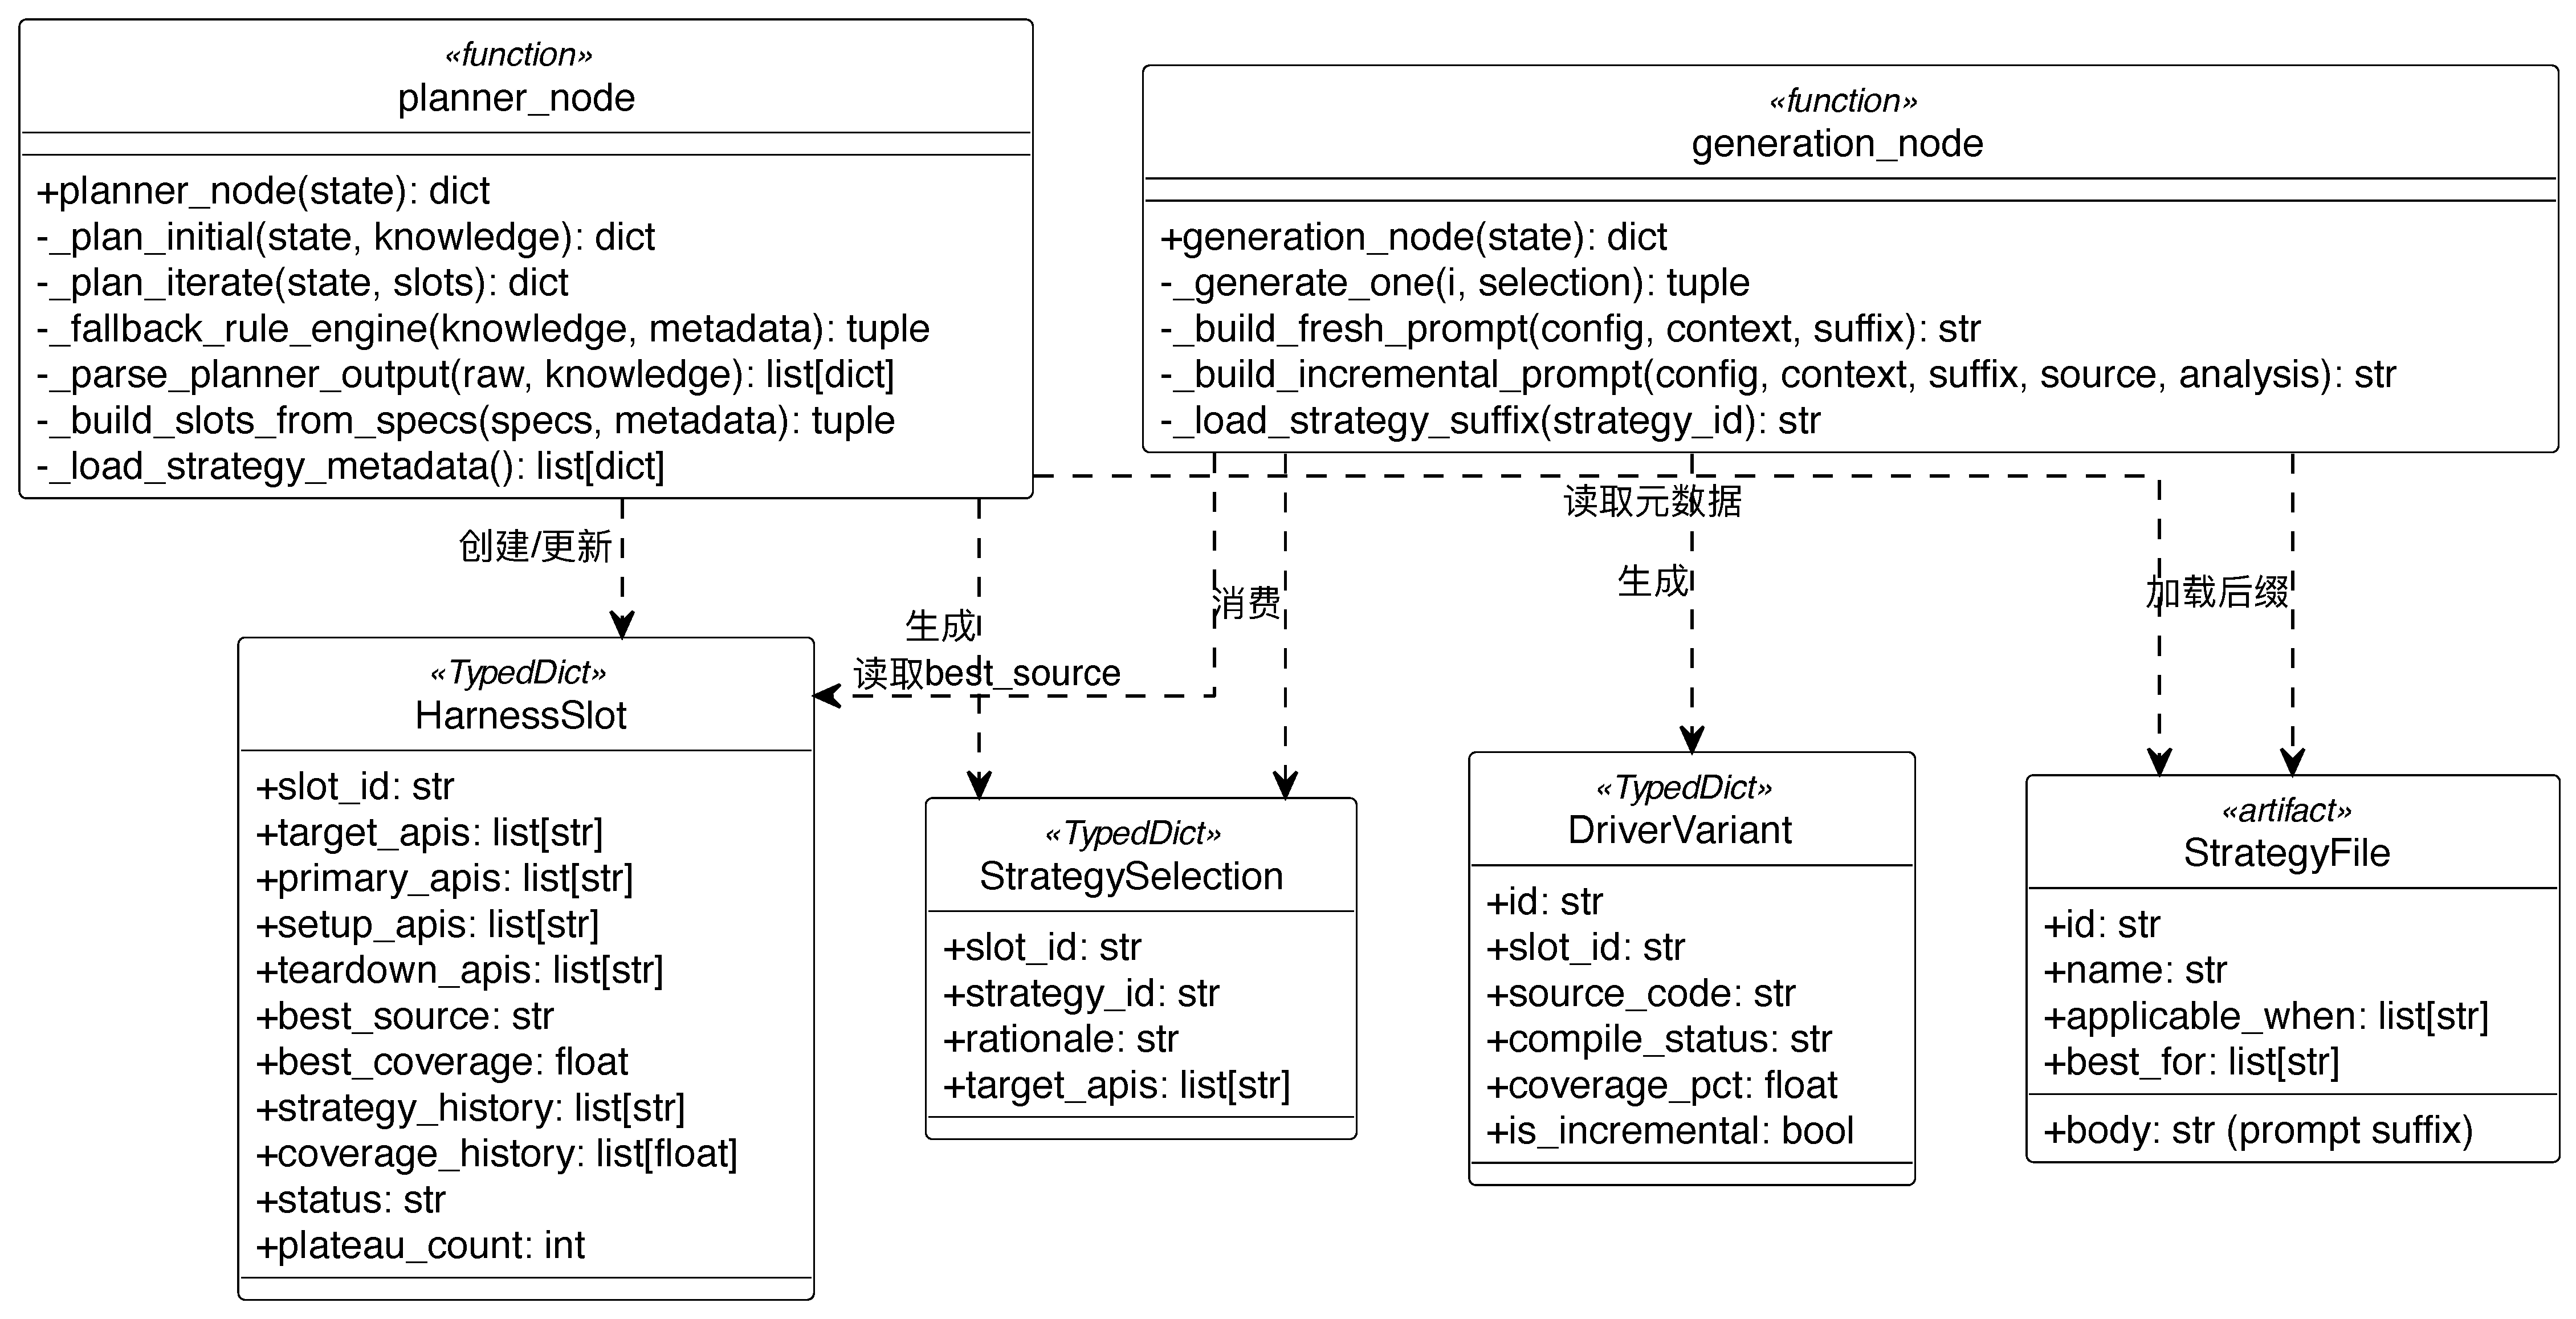
\includegraphics[width=\textwidth]{images/generation_class.pdf}
    \caption{策略规划与代码生成模块详细设计类图}
    \label{fig:generation-class}
\end{figure}

\subsection{策略规划与代码生成模块详细设计}

图\ref{fig:generation-class}展示了策略规划与代码生成模块的详细设计类图。

该模块包含两个核心函数类和四个数据类型。\texttt{planner\_node}函数类封装了策略规划的全部逻辑，公开方法\texttt{planner\_node}作为LangGraph节点入口，内部根据当前轮次分派到\texttt{\_plan\_initial}（探索阶段）或\texttt{\_plan\_iterate}（利用阶段）。\texttt{\_plan\_initial}方法承担探索阶段的核心工作：借助大语言模型进行场景推理。具体做法是将完整的API知识、调用图、类型定义注入提示词模板，由LLM分析API间的语义关系并据此设计测试场景。LLM返回的JSON结构先经\texttt{\_parse\_planner\_output}解析，再由\texttt{\_build\_slots\_from\_specs}转化为具体槽位对象。为防止LLM调用失败导致流水线中断，此处还设置了容错保障，\texttt{\_fallback\_rule\_engine}可接管工作，通过\texttt{GroupingEngine}做确定性降级。

\texttt{generation\_node}函数类封装了代码生成的全部逻辑，通过\texttt{ThreadPoolExecutor}并行调用大语言模型，为每个策略选择生成一个模糊驱动变体。内部区分两种提示词构建路径：\texttt{\_build\_fresh\_prompt}用于首轮从零生成，\texttt{\_build\_incremental\_prompt}用于后续轮次的增量改进。\texttt{\_load\_strategy\_suffix}方法从策略文件中加载YAML前置元数据之后的正文部分，作为提示词的策略后缀。

\texttt{HarnessSlot}是系统的核心状态单元，代表一个独立的模糊测试场景。每个槽位维护目标API集合（分为primary、setup、teardown三类）、历史最佳驱动源码、覆盖率历史、策略切换记录和停滞计数器。\texttt{StrategySelection}记录规划智能体为每个槽位做出的策略决策，包括策略ID、决策理由和目标API列表。\texttt{DriverVariant}记录生成智能体产出的每个驱动变体的完整信息。\texttt{StrategyFile}表示策略库中的策略文件，包含YAML前置元数据（适用条件、最佳场景）和Markdown正文（生成指导）。

图\ref{fig:generation-seq}展示了策略规划与代码生成模块的详细设计顺序图，可以看到探索阶段和利用阶段采用不同的执行路径。

\begin{figure}[H]
    \centering
    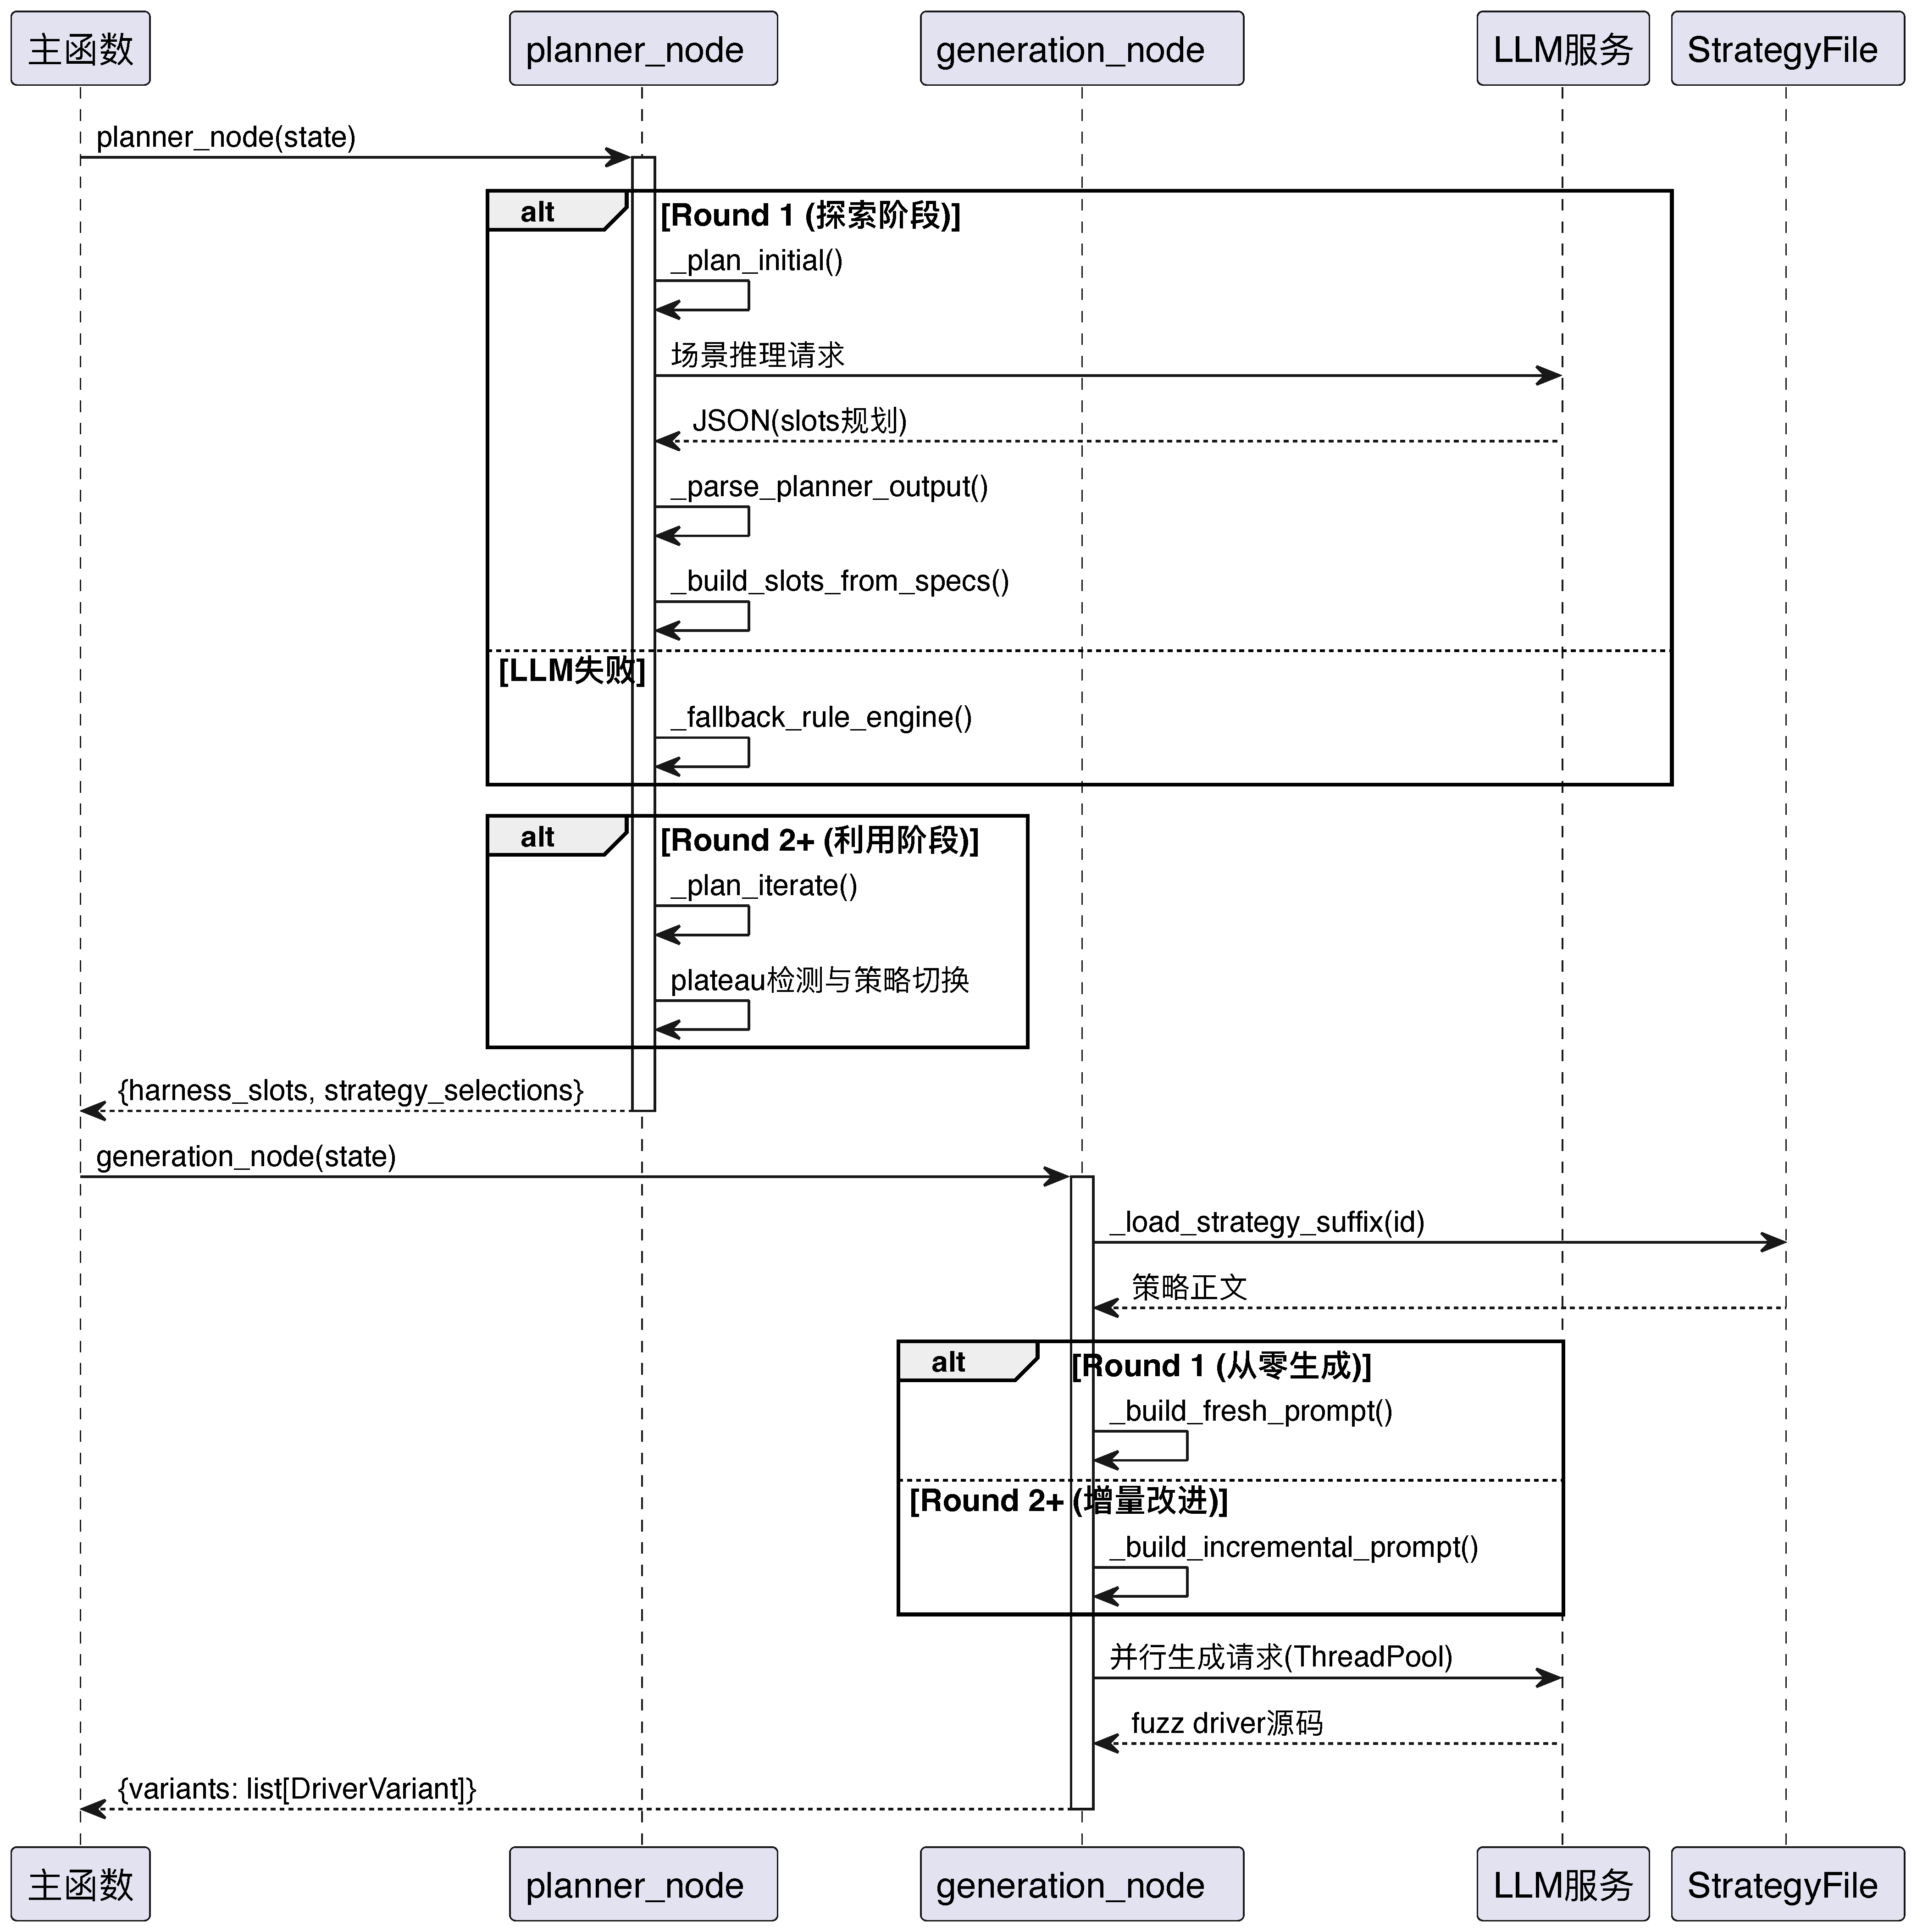
\includegraphics[width=\textwidth]{images/generation_seq.pdf}
    \caption{策略规划与代码生成模块详细设计顺序图}
    \label{fig:generation-seq}
\end{figure}

主函数先调用\texttt{planner\_node}执行策略规划。探索阶段（Round 1）的做法是把完整API知识、调用图和类型定义全部注入提示词模板，让大语言模型做场景推理。LLM返回一个JSON结构，其中包含多个槽位的规划方案。系统对其做解析校验，通过后创建\texttt{HarnessSlot}和\texttt{StrategySelection}对象。若LLM调用因网络超时或返回格式不合法而失败，则降级到规则引擎做确定性分组。进入利用阶段（Round 2+）后，规划逻辑有所不同：遍历所有活跃槽位，依据停滞计数器判断是否需要切换策略。系统设定的阈值是连续两轮覆盖率无提升则切换至\texttt{targeted-expansion}；若连续四轮仍无进展，则标记该槽位已收敛，不再投入计算资源。

随后主函数调用\texttt{generation\_node}启动代码生成。生成智能体先加载对应的策略文件后缀，然后根据当前轮次选择提示词构建路径：首轮使用三部分组装的从零生成提示词，后续轮次使用包含现有代码和诊断约束的增量改进提示词。最终通过线程池并行调用大语言模型，为每个策略选择生成一个模糊驱动变体。

\subsection{探索阶段策略规划功能实现}

这一小节解析策略规划智能体在探索阶段（Round 1）的核心实现。本节依次说明LLM场景推理、输出解析校验和确定性回退机制。

\subsubsection{LLM场景推理}

探索阶段的核心任务是将目标库的API知识转化为若干独立的模糊测试场景。系统将完整的API分类概览、调用图和类型定义注入规划提示词模板，要求大语言模型分析API间的语义关系，设计互不重叠的测试场景，并为每个场景选择最匹配的策略。\texttt{\_plan\_initial}方法的实现如图\ref{fig:plan-initial}所示。

\begin{figure}[H]
    \centering
    \begin{lstlisting}[style=style@python]
   def _plan_initial(state: PipelineState, knowledge: dict) -> dict:
       target_config = state["target_config"]
       lib_name = target_config.get("library_name", "?")
       strategy_metadata = _load_strategy_metadata()
       context = build_planner_context(knowledge, [], strategy_metadata)
       strategies_text = _format_strategies(strategy_metadata)
       prompt = PLANNER_TEMPLATE.replace("{{LIBRARY_NAME}}", lib_name)
       prompt = prompt.replace("{{KNOWLEDGE_CONTEXT}}", context)
       prompt = prompt.replace("{{CALL_GRAPH}}", _format_call_graph(knowledge))
       prompt = prompt.replace("{{TYPE_DEFINITIONS}}", _format_type_defs(knowledge))
       prompt = prompt.replace("{{STRATEGIES}}", strategies_text)
       try:
           llm = create_llm(temperature=max(state.get("temperature", 0.4) - 0.1, 0.1))
           response = llm.invoke([...])
           slot_specs = _parse_planner_output(response.content, knowledge)
           slots, selections = _build_slots_from_specs(slot_specs, strategy_metadata)
       except Exception:
           slots, selections = _fallback_rule_engine(knowledge, strategy_metadata)
       return {"harness_slots": slots, "strategy_selections": selections}
    \end{lstlisting}
    \caption{探索阶段策略规划核心流程}
    \label{fig:plan-initial}
\end{figure}

提示词组装采用模板变量替换机制，将五个知识维度注入固定模板：库名称、API知识上下文、调用图、类型定义和可用策略列表。值得注意的是温度参数的设置，比全局温度低0.1（最低0.1），目的是获得更确定性的规划输出。

\subsubsection{输出解析与校验}

大语言模型返回的规划结果为JSON格式，系统通过\texttt{\_parse\_planner\_output}方法做严格的解析和校验。实现如图\ref{fig:parse-planner}所示。

\begin{figure}[H]
    \centering
    \begin{lstlisting}[style=style@python]
   def _parse_planner_output(raw: str, knowledge: dict) -> list[dict]:
       text = raw.strip()
       match = re.search(r"```(?:json)?\s*\n(.+?)```", text, re.DOTALL)
       if match:
           text = match.group(1).strip()
       data = json.loads(text)
       slots_raw = data.get("slots", [])
       valid_apis = {a["name"] for a in knowledge.get("api_entries", [])}
       valid_strategies = {"parse-centric", "multi-api-sequence",
                           "roundtrip", "targeted-expansion", ...}
       result = []
       for spec in slots_raw:
           primary = [a for a in spec.get("primary_apis", []) if a in valid_apis]
           if not primary:
               continue
           strategy = spec.get("strategy_id", "multi-api-sequence")
           if strategy not in valid_strategies:
               strategy = "multi-api-sequence"
           result.append({...})
       return result
    \end{lstlisting}
    \caption{LLM规划输出解析与校验}
    \label{fig:parse-planner}
\end{figure}

该方法的容错设计体现在多个层面。在格式层面，它兼容两种LLM输出形式，既能从Markdown代码块中提取JSON，也能直接处理纯JSON文本。在语义层面，对API名称做有效性校验，将LLM幻觉产生的不存在函数名过滤掉。在策略层面，对策略ID做合法性检查，遇到无效策略则回退到默认的\texttt{multi-api-sequence}。经过这些校验后，只有至少包含一个有效primary API的槽位才会被保留。

\subsubsection{确定性回退机制}

当LLM调用失败时（无论是网络超时、配额耗尽还是返回格式无法解析），系统降级到基于规则引擎的确定性回退方案。这保证了流水线不会因单次LLM失败而中断。回退机制的实现如图\ref{fig:fallback-engine}所示。

\begin{figure}[H]
    \centering
    \begin{lstlisting}[style=style@python]
   def _fallback_rule_engine(knowledge: dict,
                                  strategy_metadata: list[dict]
                                  ) -> tuple[list[HarnessSlot], list[StrategySelection]]:
       groups = group_apis(knowledge, max_groups=10)
       slots: list[HarnessSlot] = []
       selections: list[StrategySelection] = []
       for i, group in enumerate(groups):
           strategy_id = match_strategy(group, strategy_metadata)
           slot_id = f"slot_{i}"
           slots.append(HarnessSlot(
               slot_id=slot_id, group_id=group["group_id"],
               target_apis=group["apis"], primary_apis=group["apis"],
               strategy_history=[strategy_id], status="active", ...
           ))
           selections.append(StrategySelection(
               slot_id=slot_id, strategy_id=strategy_id,
               target_apis=group["apis"], ...
           ))
       return slots, selections
    \end{lstlisting}
    \caption{确定性回退规则引擎}
    \label{fig:fallback-engine}
\end{figure}

回退方案调用\texttt{GroupingEngine}的\texttt{group\_apis}方法，基于调用图连通分量和参数类型相似性将API聚类为最多10个分组，再通过\texttt{match\_strategy}方法基于规则评分为每个分组匹配最适合的策略。这个方案缺乏LLM的语义推理能力，但保证了确定性和可重复性。

\subsection{多提示词策略驱动生成功能实现}

这一小节深入代码生成智能体的实现，依次说明策略文件的组织方式、三部分提示词的拼装机制以及增量改进生成的做法。

\subsubsection{策略文件结构}

MAGIC4FDG系统的策略库包含10个策略文件，每个文件采用YAML前置元数据加Markdown正文的双层结构。前置元数据定义策略的适用条件和最佳场景，供规划智能体做策略匹配；正文部分包含具体的生成指导，作为提示词后缀注入代码生成请求。表~\ref{tab:strategy-lib}列出了全部10种策略的名称、核心思路和典型适用场景。

\begin{table}[H]
    \centering
    \caption{MAGIC4FDG策略库（10种策略）}
    \makebox[\textwidth]{
    \resizebox{\textwidth}{!}{
    \begin{tabular}{|l|l|l|}
        \hline
        \textbf{策略ID} & \textbf{核心思路} & \textbf{典型适用场景} \\
        \hline
        parse-centric & 将原始模糊字节直接喂给解析API的各种变体 & 解析类库（JSON、XML、图像） \\
        \hline
        roundtrip & 解析→修改→序列化→再解析，验证往返一致性 & 序列化库（JSON、XML、YAML） \\
        \hline
        multi-api-sequence & 链式调用多个API，构造有状态的调用序列 & 数据结构库 \\
        \hline
        structure-aware & 构造符合格式规范的结构化输入 & 输入语法复杂的解析库 \\
        \hline
        stateful & 跨调用维护上下文状态，测试状态机转换 & 加密库（基于上下文的加解密） \\
        \hline
        differential & 对比同一库中不同API实现的行为差异 & 加密库（不同模式、填充方案） \\
        \hline
        targeted-expansion & 基于覆盖率反馈定向扩展未覆盖区域 & 利用阶段的增量改进 \\
        \hline
        error-path & 故意构造非法输入，覆盖错误处理路径 & 错误处理逻辑复杂的库 \\
        \hline
        callback-driven & 注册回调函数并触发事件驱动的执行路径 & 事件驱动型库 \\
        \hline
        resource-boundary & 测试内存/缓冲区边界条件和资源极限 & 压缩/解压缩库 \\
        \hline
    \end{tabular}}}
    \label{tab:strategy-lib}
\end{table}

图\ref{fig:strategy-format}展示了策略文件的结构示例。

\begin{figure}[H]
    \centering
    \begin{lstlisting}[style=style@base]
   ---
   id: parse-centric
   name: Parse-Centric Input Fuzzing
   applicable_when:
     - "library has parsing functions that accept raw bytes"
     - "API includes multiple parse variants"
   best_for:
     - "parser libraries (JSON, XML, image)"
     - "format decoders"
   ---
   ## Strategy: Parse-Centric
   Feed raw fuzz bytes directly to ALL parsing API variants.
   - Call every parse function variant
   - Use different option flag combinations
   - Exercise error paths by feeding malformed data
   - Use FuzzedDataProvider to split input
    \end{lstlisting}
    \caption{策略文件结构示例（parse-centric）}
    \label{fig:strategy-format}
\end{figure}

系统通过\texttt{\_load\_strategy\_suffix}方法加载策略正文。该方法遍历策略目录下的所有Markdown文件，通过匹配\texttt{id}字段定位目标策略，然后截取YAML前置元数据结束标记（第二个\texttt{‘---’}）之后的全部内容作为策略后缀。

\subsubsection{从零生成提示词组装}

首轮生成采用三部分组装机制构建提示词：基础模板提供通用的生成框架和约束，知识上下文提供目标API的详细信息，策略后缀提供特定策略的生成指导。\texttt{\_build\_fresh\_prompt}方法的实现如图\ref{fig:fresh-prompt}所示。

\begin{figure}[H]
    \centering
    \begin{lstlisting}[style=style@python]
   def _build_fresh_prompt(target_config: dict, knowledge_context: str,
                                strategy_suffix: str) -> str:
       include_dirs = target_config.get("include_dirs", [])
       prompt = (
           GENERATION_TEMPLATE
           .replace("{{LIBRARY_NAME}}", target_config.get("library_name", ""))
           .replace("{{LANGUAGE}}", target_config.get("language", "C"))
           .replace("{{HEADER}}", target_config.get("header", ""))
           .replace("{{INCLUDE_DIRS}}", ", ".join(include_dirs))
           .replace("{{RESEARCH_SUMMARY}}", knowledge_context)
           .replace("{{COVERAGE_FEEDBACK}}", "(first round)")
       )
       if strategy_suffix:
           prompt += "\n\n" + strategy_suffix
       return prompt
    \end{lstlisting}
    \caption{从零生成提示词三部分组装}
    \label{fig:fresh-prompt}
\end{figure}

基础模板\texttt{GENERATION\_TEMPLATE}对模糊驱动提出了若干通用约束：必须包含\texttt{LLVMFuzzerTestOneInput}入口函数，头文件引用路径正确，资源管理需满足内存安全。知识上下文由\texttt{build\_generator\_context}方法构建，涵盖目标API的完整签名、参数语义、类型定义和宏常量。策略后缀则给出特定测试策略的具体指导，以\texttt{parse-centric}策略为例，它会要求"把原始模糊字节直接喂给所有解析API变体"。三部分各有侧重，拼合后形成完整的生成请求。

\subsubsection{增量改进提示词组装}

第二轮及之后的迭代采用增量改进模式，基于该槽位的历史最佳驱动做修改，而非从零重新生成。这样做的好处是保留了已有的覆盖率成果，同时针对诊断智能体识别的覆盖率缺口做定向改进。\texttt{\_build\_incremental\_prompt}方法的实现如图\ref{fig:incremental-prompt}所示。

\begin{figure}[H]
    \centering
    \begin{lstlisting}[style=style@python]
   def _build_incremental_prompt(target_config: dict, knowledge_context: str,
                                       strategy_suffix: str, base_source: str,
                                       coverage_analysis: dict) -> str:
       constraints_text = ""
       if coverage_analysis:
           constraints = coverage_analysis.get("constraints", [])
           if constraints:
               constraints_text = "\n".join(
                   f"- {c.get('target', '?')}: {c.get('precondition', '')}"
                   for c in constraints[:10])
       clusters_text = ""
       if coverage_analysis:
           clusters = coverage_analysis.get("uncovered_clusters", [])
           if clusters:
               clusters_text = "\n".join(
                   f"- {', '.join(c.get('functions', []))}: {c.get('root_cause', '')}"
                   for c in clusters[:5])
       prompt = f"""## Task: Improve Fuzz Driver
                      ## Current Driver (to be improved)
                      ```cpp
                      {base_source}
                      ```
                      ## Analyst Constraints
                      {constraints_text or "(no specific constraints)"}
                      ## Uncovered Code Clusters
                      {clusters_text or "(no cluster data)"}
                      ## API Knowledge
                      {knowledge_context}
                      ## Strategy Guidance
                      {strategy_suffix}"""
       return prompt
    \end{lstlisting}
    \caption{增量改进提示词组装}
    \label{fig:incremental-prompt}
\end{figure}

增量提示词分五个层次组织信息。最上面放现有驱动源码，作为修改的基础。然后是诊断约束，最多放10条，每条指明需要覆盖的具体目标和前置条件。接着是未覆盖代码簇，最多5个，附带根因分析。再往下是API知识上下文和策略指导。提示词中明确指定了"保留现有驱动中有效的部分，仅添加新的代码路径"，这一步至关重要，否则大语言模型容易将已有的覆盖率成果破坏。

\section{模糊测试与覆盖率收集模块详细设计与实现}

模糊测试与覆盖率收集模块构成了MAGIC4FDG系统的执行层与反馈源。它负责在Docker容器内运行生成的模糊驱动、收集细粒度代码覆盖率数据，并借助控制流图可达性分析剔除结构性不可达的代码路径。该模块的输出直接驱动系统的迭代决策——覆盖率提升则继续优化，停滞则切换策略或终止。本节先通过类图和顺序图阐述模块的详细设计，再分别解析Fork模式模糊测试与语料库重放、控制流图可达性分析两个核心功能的实现。

\subsection{模糊测试与覆盖率收集模块详细设计}

图\ref{fig:coverage-class}展示了模糊测试与覆盖率收集模块的详细设计类图。

\begin{figure}[H]
    \centering
    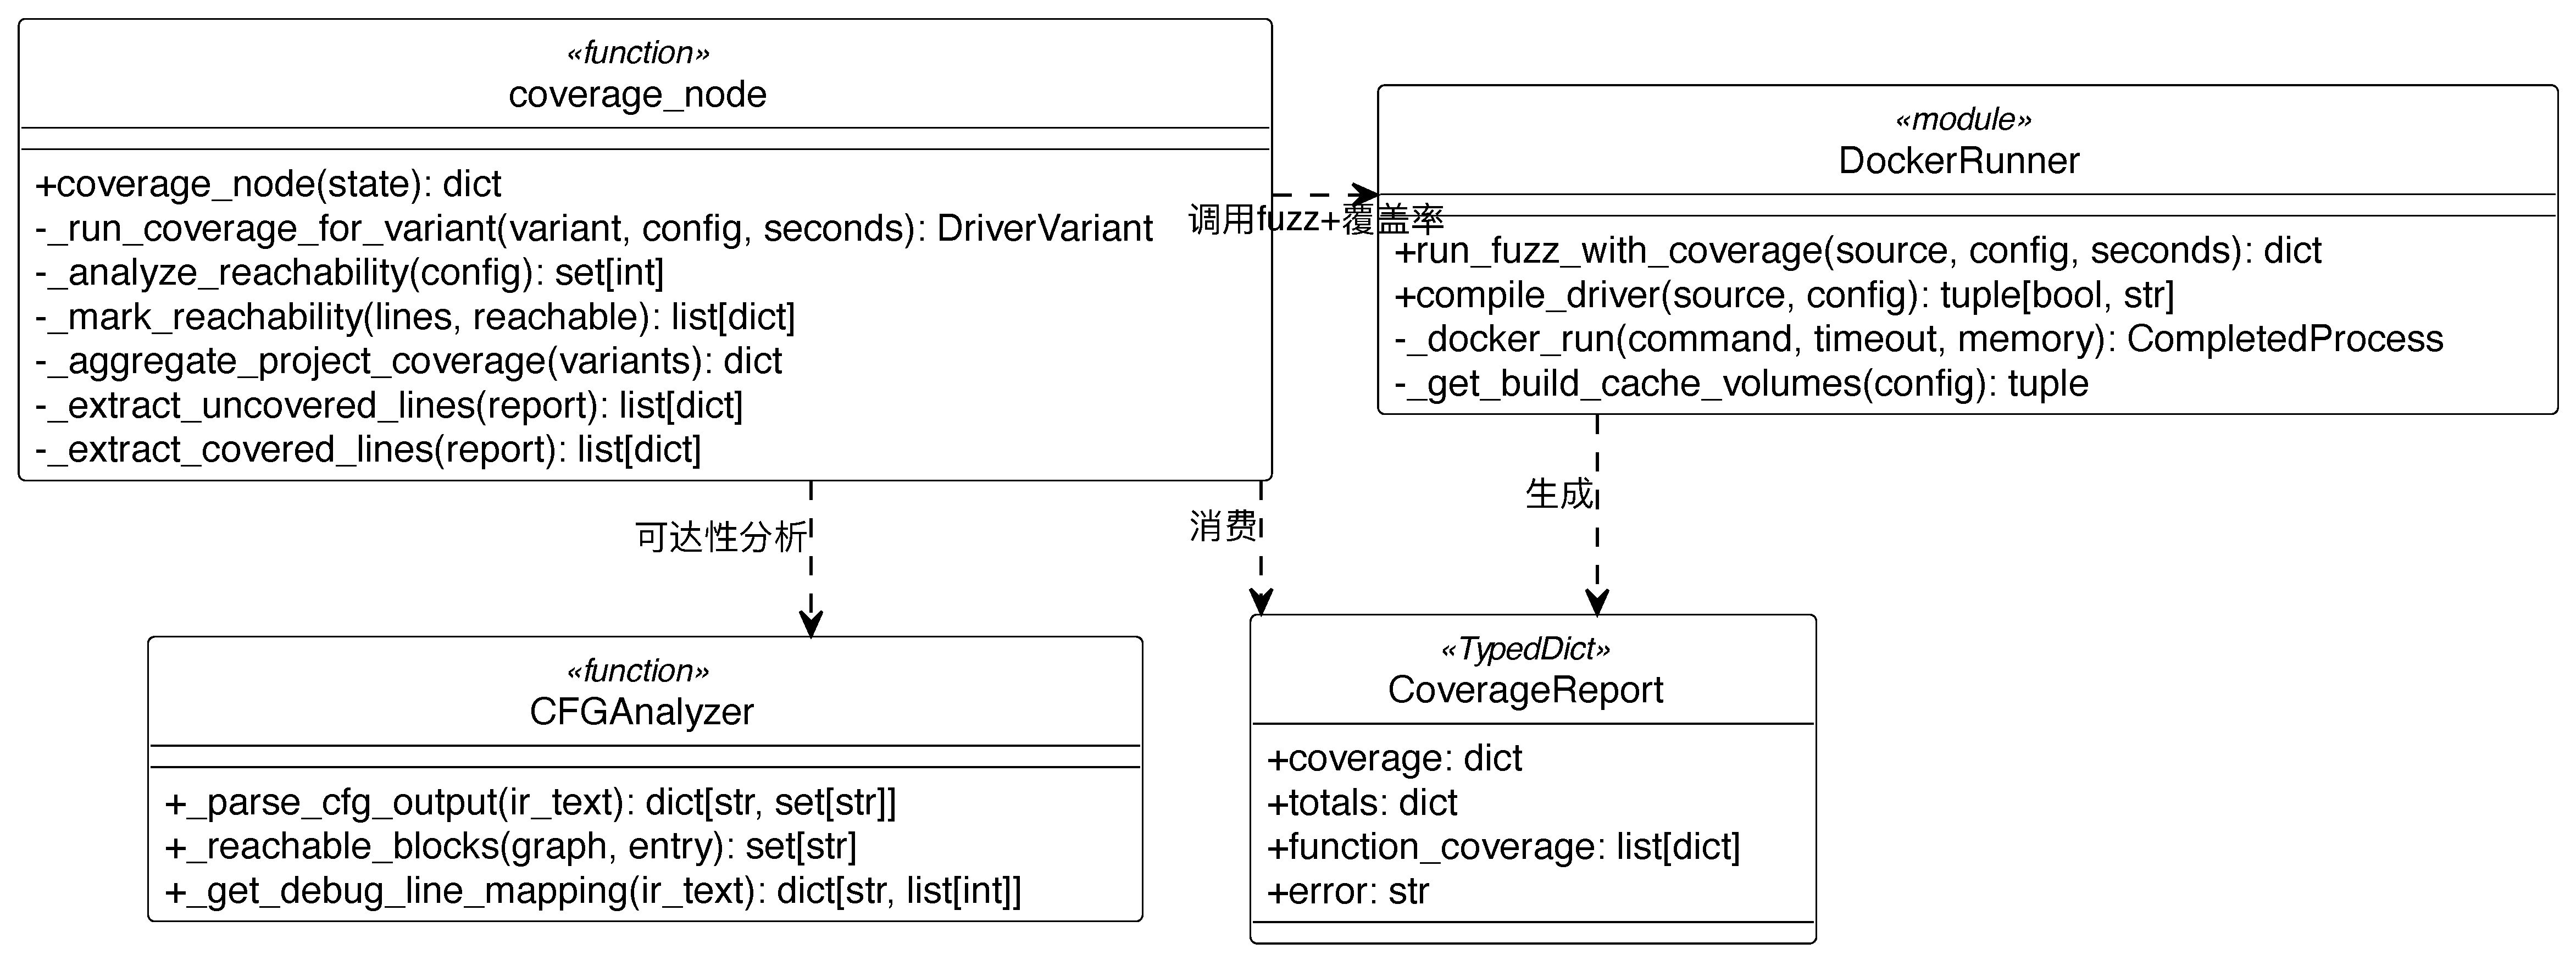
\includegraphics[width=\textwidth]{images/coverage_class.pdf}
    \caption{模糊测试与覆盖率收集模块详细设计类图}
    \label{fig:coverage-class}
\end{figure}

该模块包含三个核心组件，各负责一项独立职能。\texttt{coverage\_node}函数类是LangGraph节点入口，它编排整个流程：先执行可达性分析获取可达行集合，然后开启线程池并行对所有编译成功的变体做模糊测试，最后更新各槽位的覆盖率状态、聚合出项目级覆盖率。\texttt{DockerRunner}模块封装了Docker容器内的全部执行操作，核心方法\texttt{run\_fuzz\_with\_coverage}采用从编译到覆盖率导出的完整八步流水线。\texttt{CFGAnalyzer}组件负责基于LLVM IR的控制流图可达性分析，内部拆分为CFG解析、BFS遍历、调试信息行号映射三个子功能。

\texttt{CoverageReport}记录单个变体的覆盖率收集结果，包含行覆盖率、分支覆盖率、函数覆盖率和未覆盖行列表。值得注意的是，每个未覆盖行条目都附带一个\texttt{reachable}字段，标明该行从驱动入口函数出发是否结构性可达。

图\ref{fig:coverage-seq}展示了模糊测试与覆盖率收集模块的详细设计顺序图。

\begin{figure}[H]
    \centering
    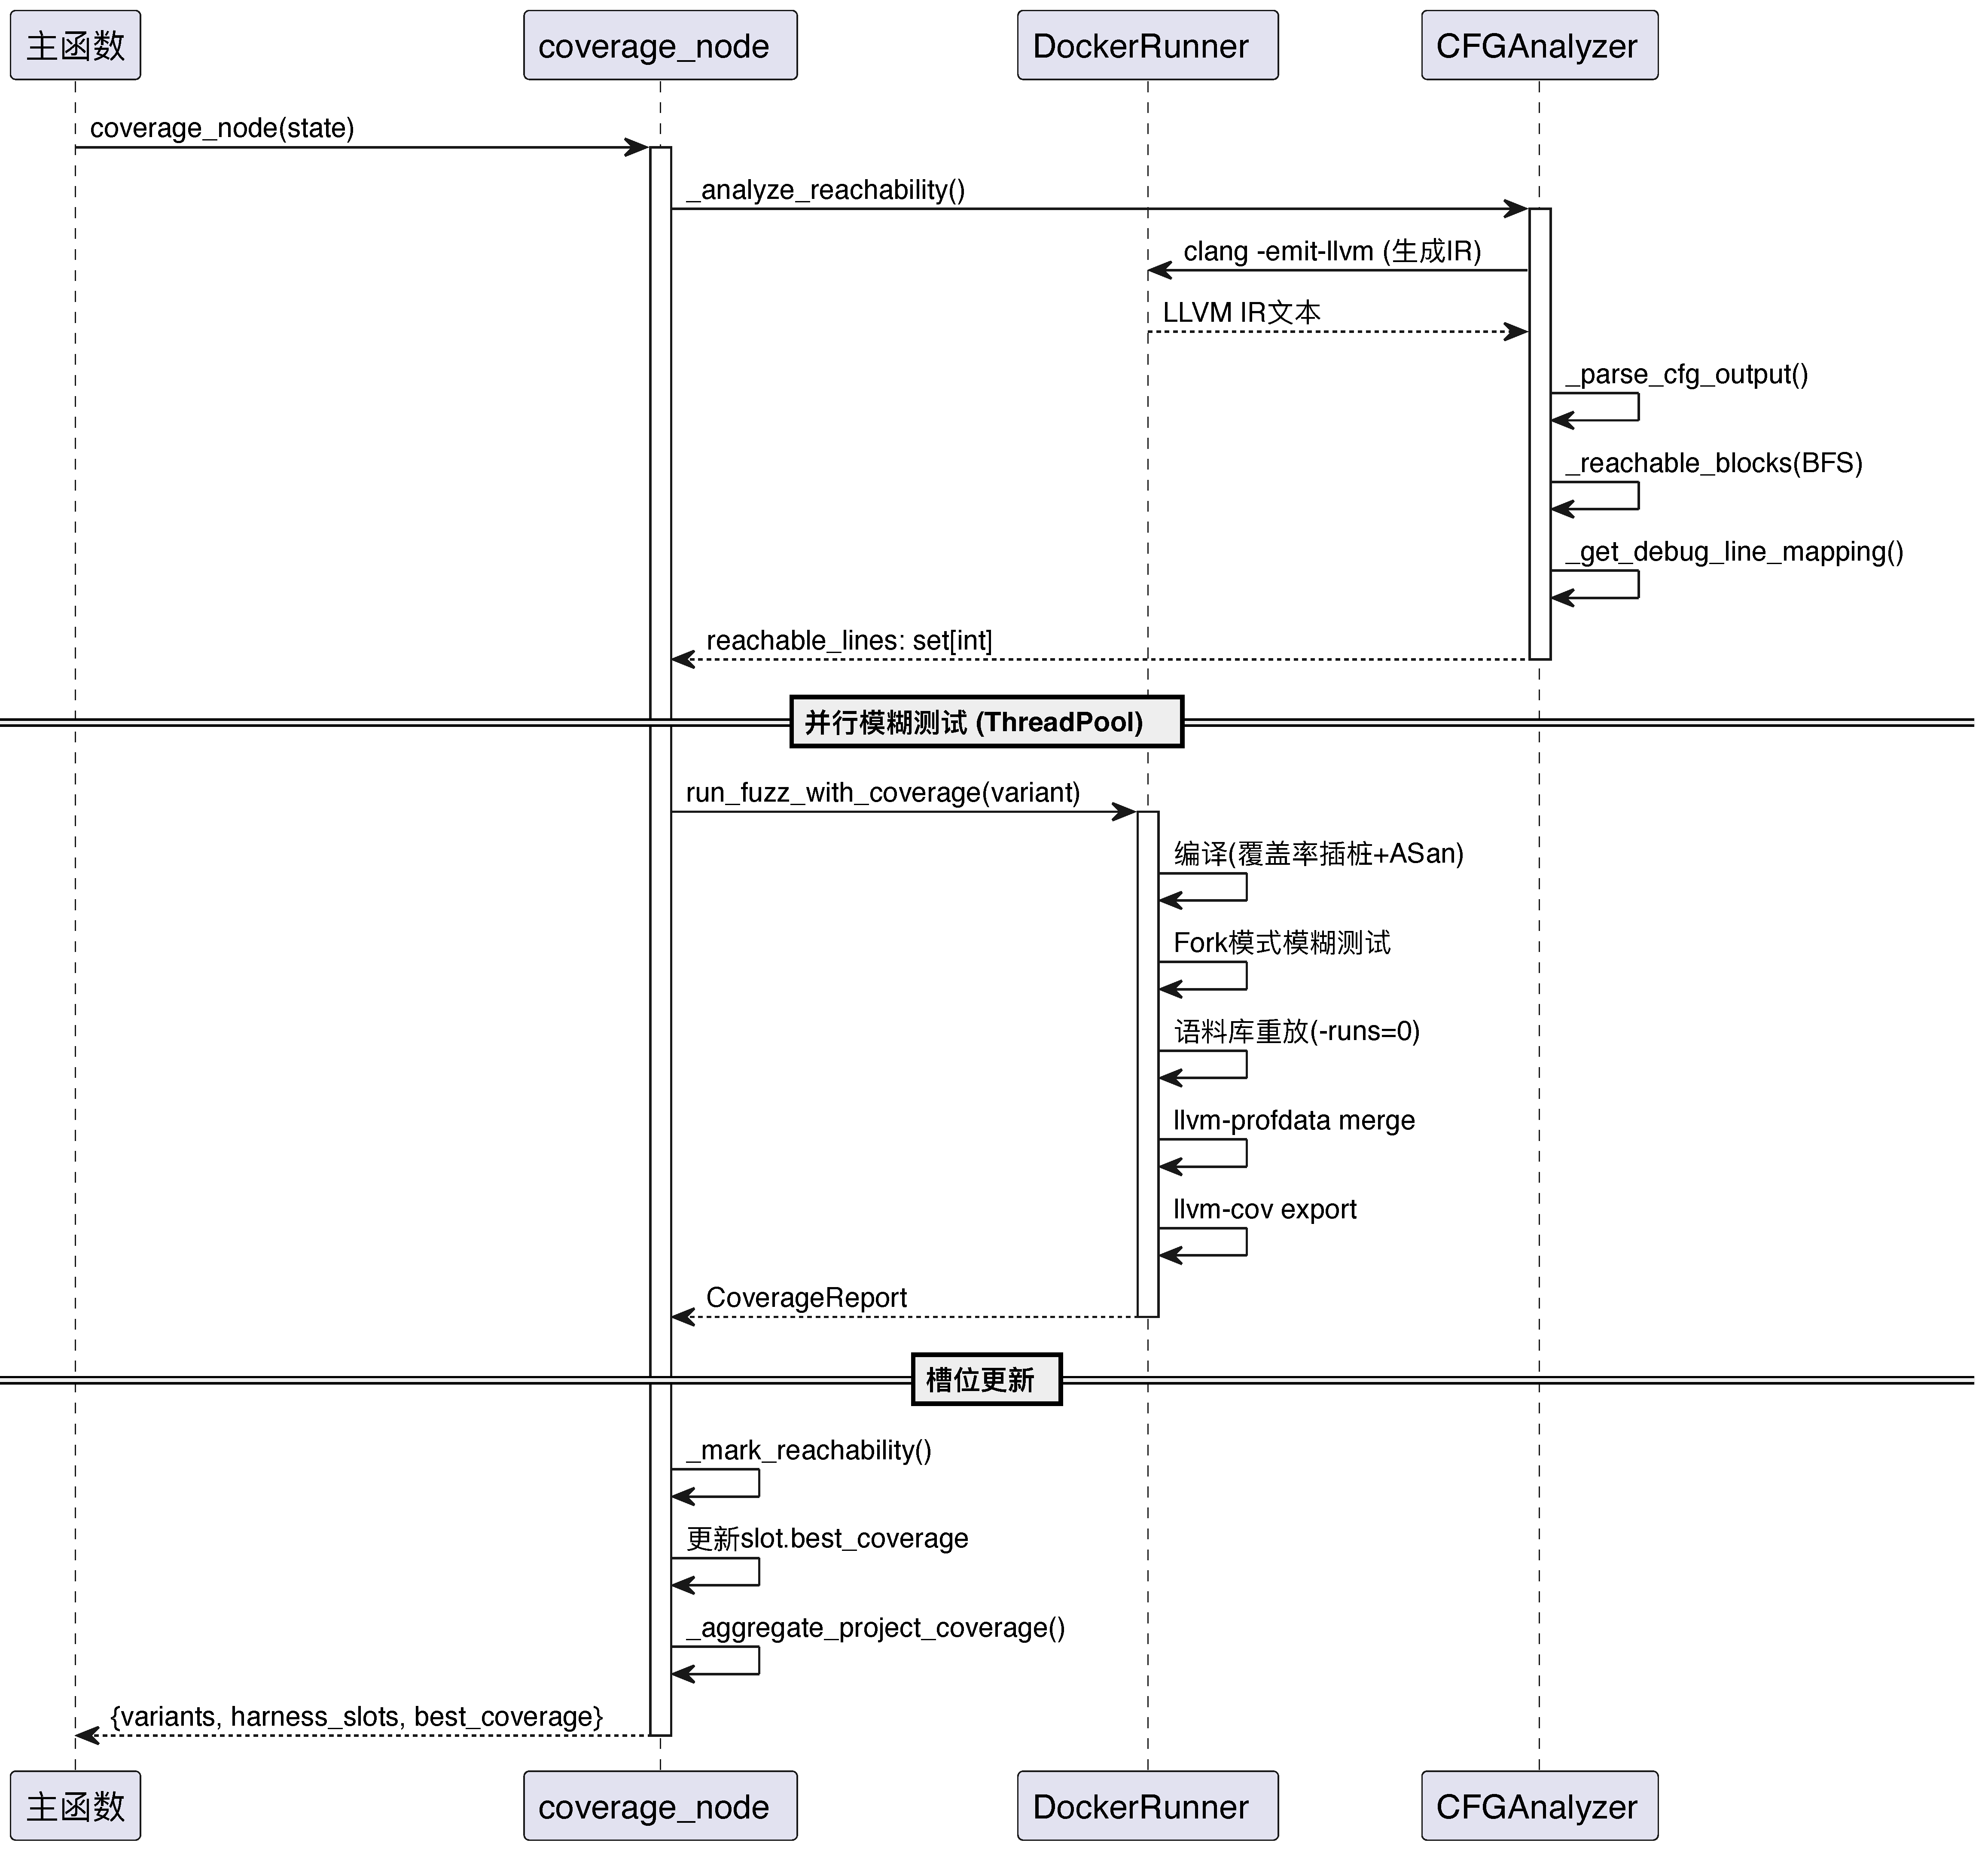
\includegraphics[width=\textwidth]{images/coverage_seq.pdf}
    \caption{模糊测试与覆盖率收集模块详细设计顺序图}
    \label{fig:coverage-seq}
\end{figure}

主函数调用\texttt{coverage\_node}后，流程分为两大步骤。第一步是可达性分析：在Docker容器内用\texttt{clang -emit-llvm}生成LLVM IR，解析IR文本构建控制流图，从入口块执行BFS获取可达基本块集合，再通过调试信息将可达块映射回源码行号。第二步是实际的模糊测试：节点开启线程池，并行调用\texttt{DockerRunner}的\texttt{run\_fuzz\_with\_coverage}方法，每个编译成功的变体都经历完整的八步流水线。执行完毕后，节点为每个未覆盖行标注可达性信息，更新各槽位的最佳覆盖率和停滞计数器，最后将所有槽位覆盖行取并集计算出项目级覆盖率。

\subsection{Fork模式模糊测试与语料库重放功能实现}

这一小节解析\texttt{run\_fuzz\_with\_coverage}方法实现的八步覆盖率收集流水线。本节重点说明Fork模式崩溃隔离和语料库重放的设计动机与实现细节。

\subsubsection{八步流水线设计}

覆盖率收集流水线在单个Docker容器内依次执行八个步骤，其核心流程如图\ref{fig:fuzz-pipeline}所示。

\begin{figure}[H]
    \centering
    \begin{lstlisting}[style=style@base]
   # Step 1: 编译(覆盖率插桩 + ASan)
   COMMON_FLAGS="-g -O1 -fprofile-instr-generate -fcoverage-mapping
                 -fsanitize=address"
   clang++ $COMMON_FLAGS driver.cpp -fsanitize=fuzzer,address -o fuzz_cov

   # Step 2: 准备语料库(种子 + 累积)
   mkdir -p /tmp/corpus && cp seed_corpus/* /tmp/corpus/
   cp accumulated_corpus/* /tmp/corpus/

   # Step 3: Fork模式模糊测试(崩溃隔离)
   export ASAN_OPTIONS=halt_on_error=0:exitcode=0:detect_leaks=0
   ./fuzz_cov /tmp/corpus -max_total_time=60 -fork=1

   # Step 4: 保存累积语料库
   cp /tmp/corpus/* accumulated_corpus/

   # Step 5: 语料库重放(无Fork, 收集完整profraw)
   export LLVM_PROFILE_FILE=/tmp/replay_%m.profraw
   ./fuzz_cov /tmp/corpus -runs=0

   # Step 6: 合并覆盖率数据
   llvm-profdata merge -sparse /tmp/replay_*.profraw -o fuzzer.profdata

   # Step 7: 导出覆盖率报告(JSON)
   llvm-cov export ./fuzz_cov -instr-profile=fuzzer.profdata sources

   # Step 8: 导出函数级报告
   llvm-cov report ./fuzz_cov -instr-profile=fuzzer.profdata sources
    \end{lstlisting}
    \caption{八步覆盖率收集流水线}
    \label{fig:fuzz-pipeline}
\end{figure}

\subsubsection{Fork模式崩溃隔离}

LibFuzzer的Fork模式（\texttt{-fork=1}）将每个模糊输入在独立子进程中执行。当AddressSanitizer检测到内存错误时，仅子进程被终止，主进程继续运行后续输入。这一机制对覆盖率收集至关重要，若不使用Fork模式，单次ASan崩溃就会终止整个模糊测试进程，后续输入无法执行，覆盖率数据严重不完整。系统同时设置\texttt{ASAN\_OPTIONS=halt\_on\_error=0:exitcode=0:detect\_leaks=0}，确保即使在非Fork模式的重放阶段，ASan错误也不会中断执行。

\subsubsection{语料库重放设计动机}

Fork模式存在一个固有缺陷：子进程在超时时被\texttt{SIGKILL}强制终止，\texttt{profraw}覆盖率数据文件来不及刷新到磁盘。这一技术细节需要说明：Fork模式下子进程超时会被\texttt{SIGKILL}强制终止，\texttt{profraw}覆盖率文件无法正常落盘。因此系统在Fork模式执行完毕后，额外增加了一次无Fork模式的语料库重放（\texttt{-runs=0}）。重放阶段使用独立的\texttt{LLVM\_PROFILE\_FILE}路径，\texttt{llvm-profdata merge}合并时优先取重放产生的完整数据。本质上这是"先Fork后重放"的两阶段设计，Fork保证崩溃不会打断测试，重放保证覆盖率数据的完整性。

另外系统还做了跨轮次的语料库累积：每轮测试结束后把新发现的语料库文件存到持久化目录，下一轮启动时自动加载作为初始种子。这样后续轮次就能在前面的探索基础上继续深入，不用重复走已知路径。

\subsection{控制流图可达性分析功能实现}

这一小节解析基于LLVM IR的控制流图可达性分析实现。该分析用于过滤结构性不可达的未覆盖代码行，避免诊断智能体在无法通过任何输入触达的代码路径上浪费推理资源。

\subsubsection{LLVM IR生成与CFG解析}

可达性分析的第一步是在Docker容器内通过\texttt{clang -S -emit-llvm -g -O0}将目标源文件编译为LLVM中间表示（IR），保留完整的调试信息。然后系统解析IR文本构建控制流图。CFG解析的核心实现如图\ref{fig:parse-cfg}所示。

\begin{figure}[H]
    \centering
    \begin{lstlisting}[style=style@python]
   def _parse_cfg_output(cfg_text: str) -> dict[str, set[str]]:
       graph: dict[str, set[str]] = {}
       current_block = None
       for line in cfg_text.splitlines():
           block_match = re.match(r"^(\S+):.*$", line.strip())
           if block_match:
               current_block = block_match.group(1)
               if current_block not in graph:
                   graph[current_block] = set()
               continue
           if current_block:
               br_match = re.match(r"\s*br\s+.*label\s+%(\S+)", line)
               if br_match:
                   targets = re.findall(r"label\s+%([A-Za-z0-9_.]+)", line)
                   for t in targets:
                       graph[current_block].add(t)
                       if t not in graph:
                           graph[t] = set()
       return graph
    \end{lstlisting}
    \caption{LLVM IR控制流图解析}
    \label{fig:parse-cfg}
\end{figure}

该方法逐行扫描LLVM IR文本，通过正则表达式识别两类关键结构：基本块标签（行首非空白字符后跟冒号）和分支指令（\texttt{br}指令中的\texttt{label}目标）。解析结果为邻接表形式的有向图，每个节点为基本块标签，边表示控制流转移关系。

\subsubsection{BFS可达性遍历与行号映射}

获取CFG后，系统从入口基本块出发执行广度优先搜索，确定所有从程序入口可达的基本块。然后通过LLVM IR中的\texttt{!dbg}调试元数据，将可达基本块映射到对应的源码行号。可达性分析的完整流程如图\ref{fig:reachability}所示。

\texttt{\_get\_debug\_line\_mapping}方法通过两阶段处理建立基本块到源码行的映射。第一阶段扫描IR末尾的\texttt{!DILocation}元数据定义，建立元数据ID到行号的索引。第二阶段遍历函数体中每条指令的\texttt{!dbg}引用，将行号归属到对应的基本块。最终，\texttt{\_mark\_reachability}方法将可达性信息标注到每个未覆盖行条目的\texttt{reachable}字段中。诊断智能体仅对\texttt{reachable=True}的未覆盖行做分析，有效避免了在死代码和编译器生成的不可达路径上浪费推理资源。

\begin{figure}[H]
    \centering
    \begin{lstlisting}[style=style@python]
   def _analyze_reachability(target_config: dict) -> set[int]:
       source_files = target_config.get("source_files", [])
       if not source_files:
           return set()
       primary_source = source_files[0]
       include_args = " ".join(f"-I{d}" for d in target_config.get("include_dirs", []))
       # Docker内生成LLVM IR
       result = _docker_run(["bash", "reachability_analysis.sh"])
       ir_text = result.stdout
       # 解析CFG并执行BFS
       graph = _parse_cfg_output(ir_text)
       entry = "entry" if "entry" in graph else next(iter(graph), "")
       reachable = _reachable_blocks(graph, entry)
       # 映射到源码行号
       block_to_lines = _get_debug_line_mapping(ir_text)
       reachable_lines: set[int] = set()
       for block_label in reachable:
           reachable_lines.update(block_to_lines.get(block_label, []))
       return reachable_lines
    \end{lstlisting}
    \caption{控制流图可达性分析完整流程}
    \label{fig:reachability}
\end{figure}

\section{缺口诊断模块详细设计与实现}

缺口诊断模块在整个迭代闭环中承担的职责是诊断覆盖率缺口。它分析每个槽位的覆盖率数据，识别哪些代码未被覆盖以及未覆盖的原因，然后输出结构化的改进约束供下一轮代码生成使用。设计中遵循的一个核心原则是按槽位隔离：每个槽位只分析自身职责范围内的覆盖率，不涉及其他槽位的内容。这样做是为了避免跨槽位的错误引导，比如解析场景的诊断结果不应影响生命周期管理场景的生成。本节先用类图和顺序图说明设计，再分别展开覆盖率缺口诊断和跨轮次知识累积的实现。

\subsection{缺口诊断模块详细设计}

图\ref{fig:analyst-class}展示了缺口诊断模块的详细设计类图。

\texttt{analyst\_node}函数类是模块的驱动核心，其公开方法作为LangGraph节点入口，内部借助线程池对每个活跃槽位并行调用\texttt{\_analyze\_single\_slot}方法完成独立诊断。诊断过程中，\texttt{ContextBuilder}模块负责构建诊断上下文，\texttt{\_build\_uncovered\_summary}和\texttt{\_build\_function\_summary}两个辅助方法则将覆盖率数据转换为大语言模型可理解的文本形式。LLM返回的文本由\texttt{\_parse\_analyst\_response}方法提取其中的JSON结构化分析结果。

\begin{figure}[H]
    \centering
    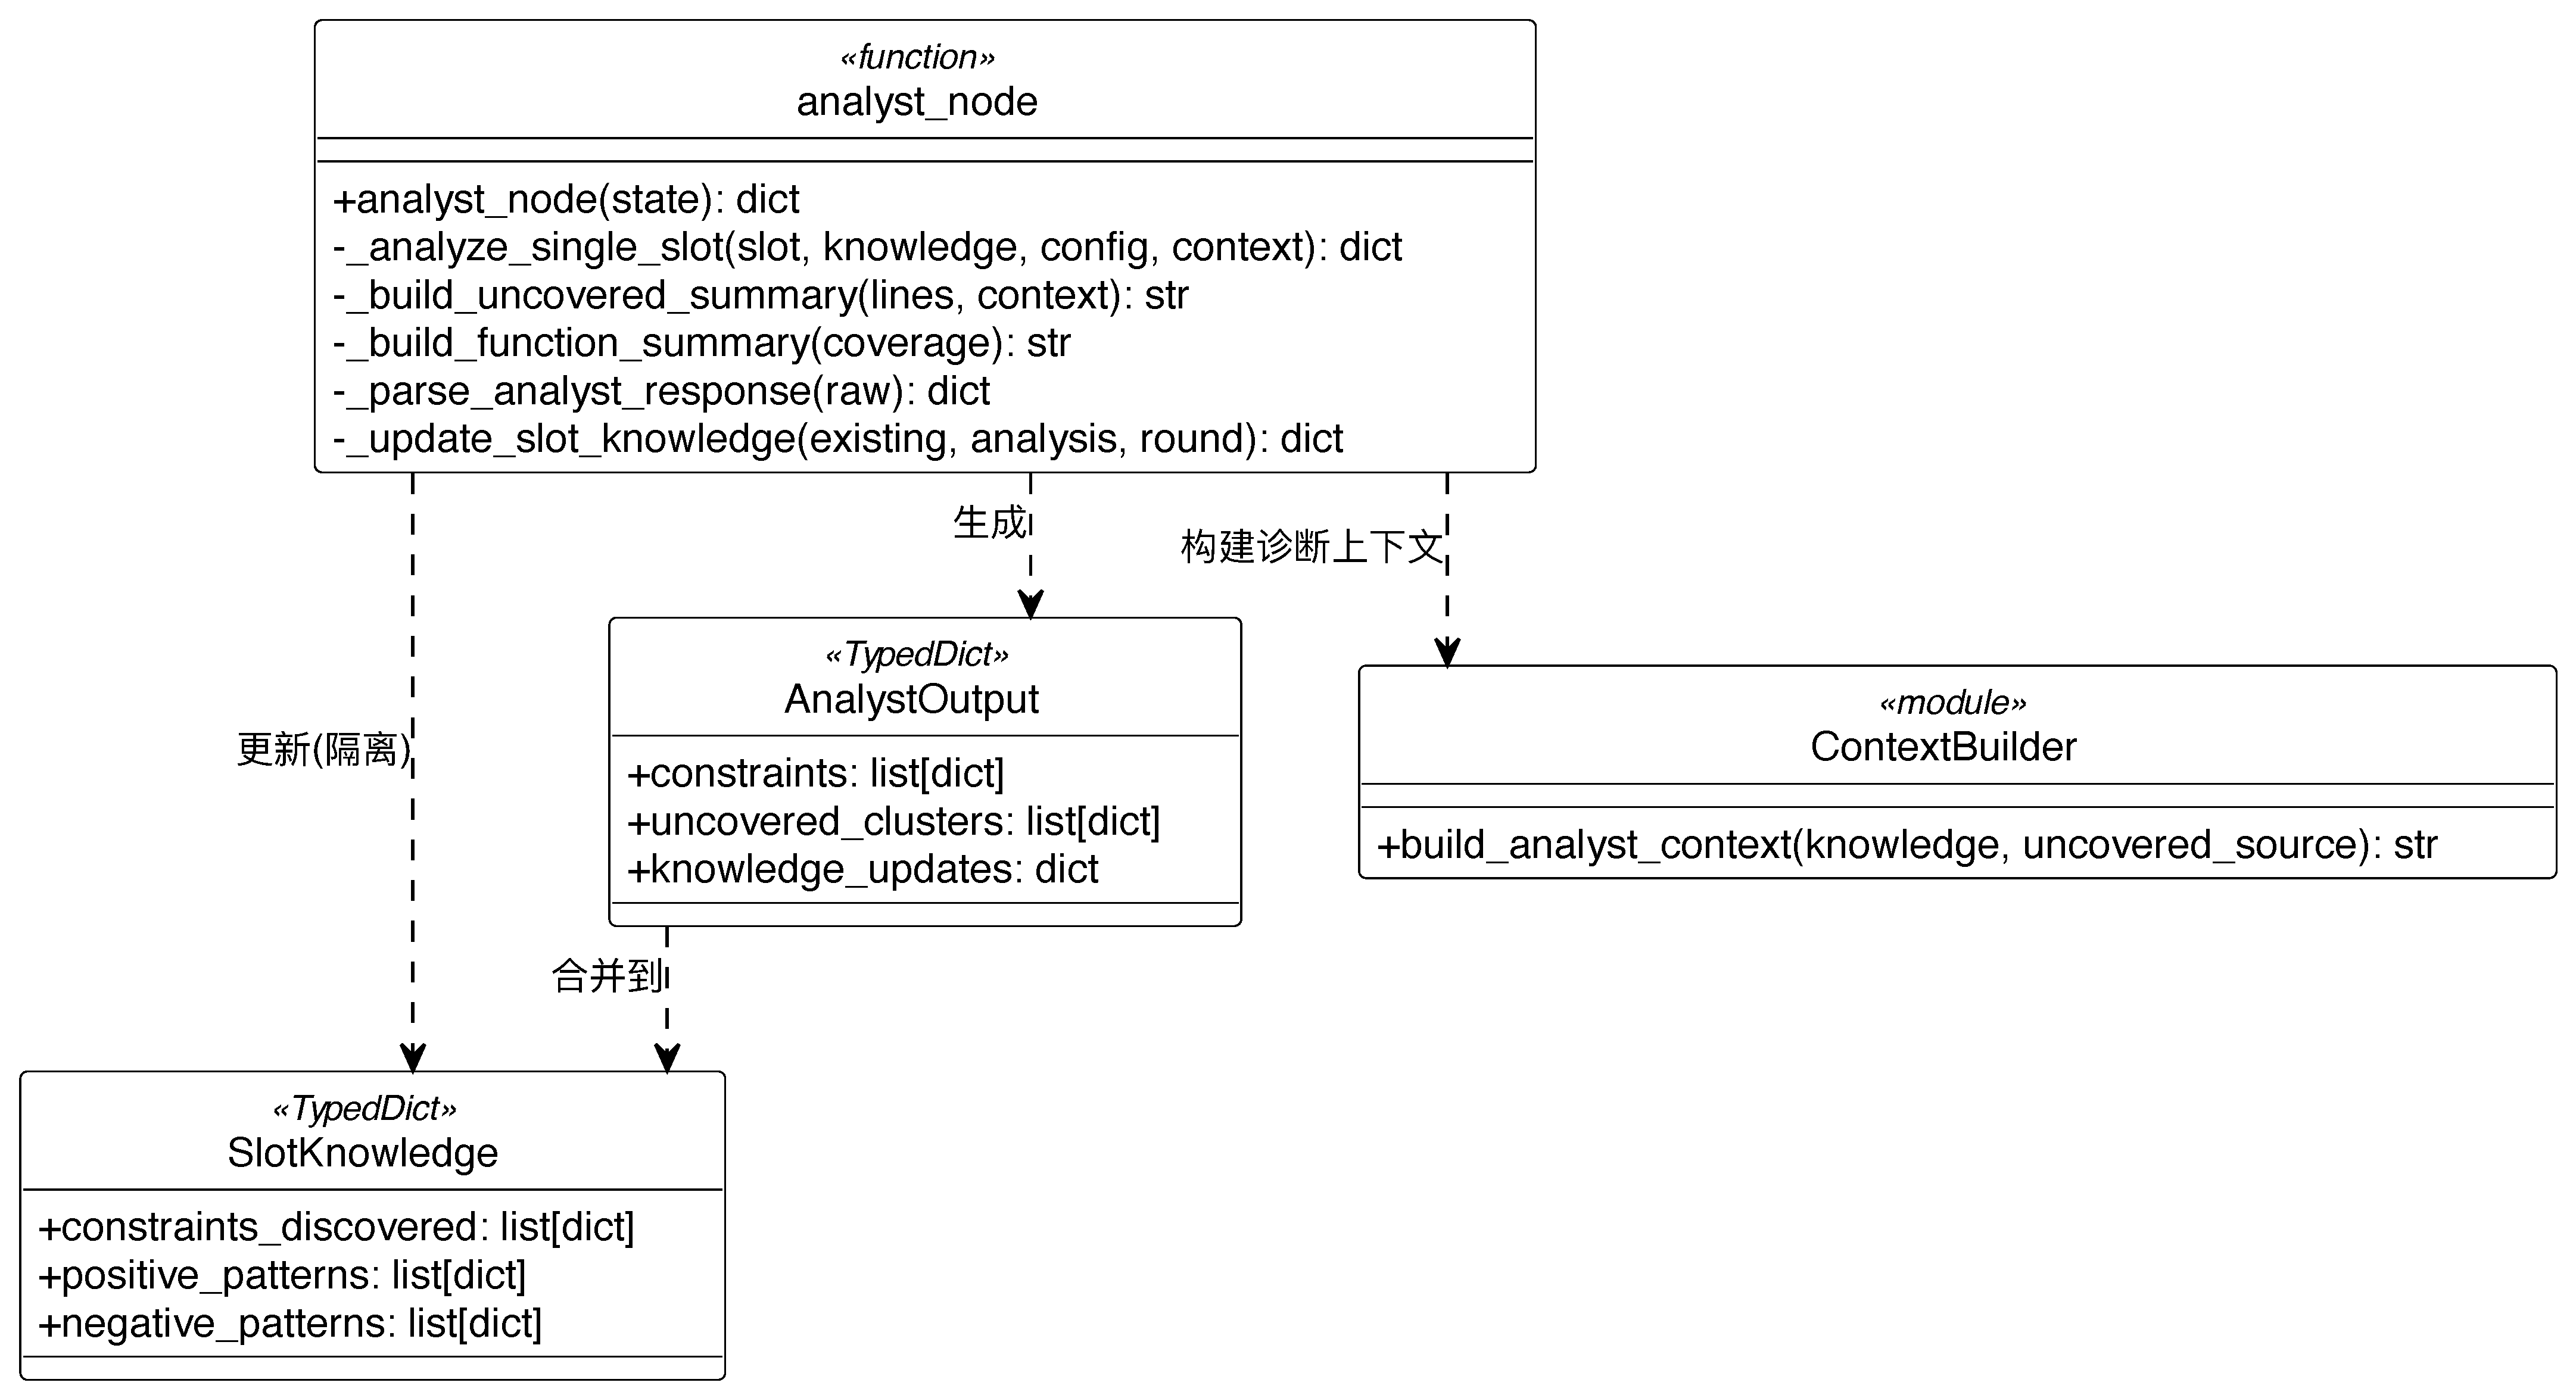
\includegraphics[width=\textwidth]{images/analyst_class.pdf}
    \caption{缺口诊断模块详细设计类图}
    \label{fig:analyst-class}
\end{figure}

\texttt{AnalystOutput}记录单次诊断的输出，包含三个字段：\texttt{constraints}列出需要满足的前置条件和目标API；\texttt{uncovered\_clusters}将未覆盖行按根因聚类；\texttt{knowledge\_updates}包含本轮发现的新约束和模式。\texttt{SlotKnowledge}是每个槽位的隔离知识空间，累积存储历史轮次发现的约束、正向模式和负向模式，供后续轮次的代码生成智能体参考。

图\ref{fig:analyst-seq}展示了缺口诊断模块的详细设计顺序图。

主函数调用\texttt{analyst\_node}启动诊断流程。该节点先筛选所有状态为\texttt{active}的槽位，然后通过线程池并行执行每个槽位的独立分析。对于每个槽位，系统构建包含完整API清单和未覆盖源码行的诊断上下文，组装诊断提示词后调用大语言模型做推理，解析返回的JSON结构化结果。最后，系统将诊断发现合并到该槽位的隔离知识空间中，并递增轮次计数器。

\begin{figure}[H]
    \centering
    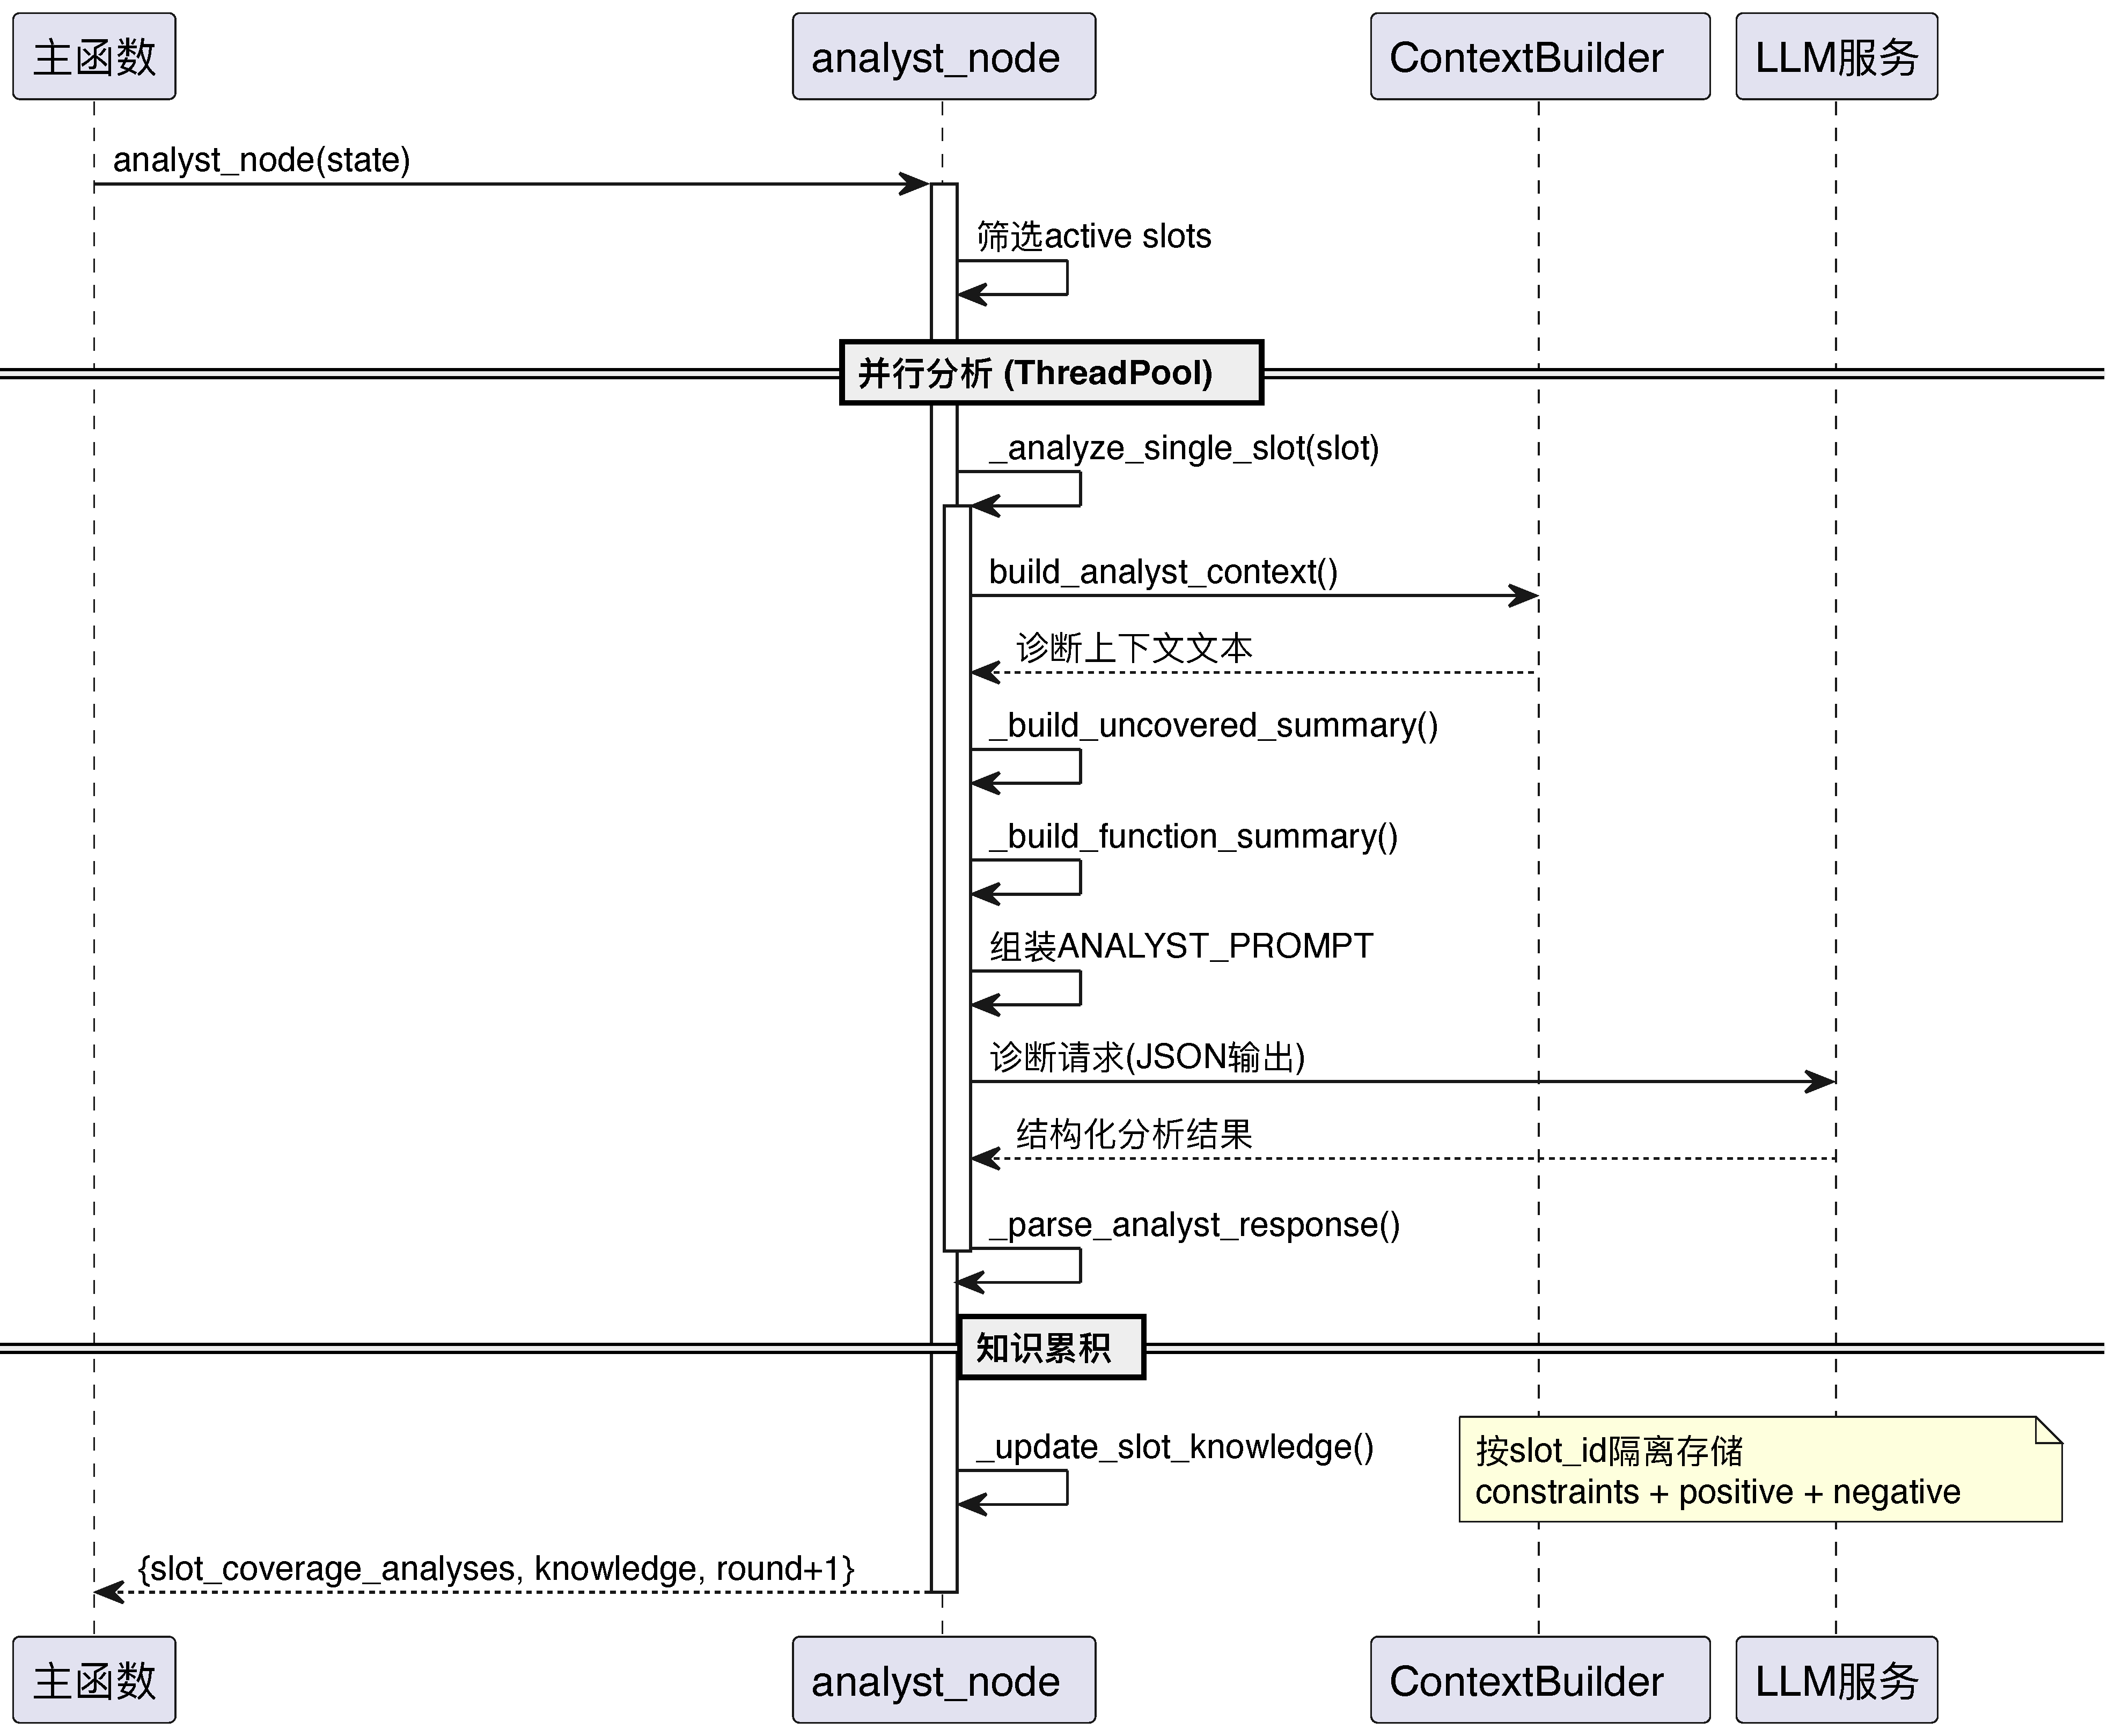
\includegraphics[width=\textwidth]{images/analyst_seq.pdf}
    \caption{缺口诊断模块详细设计顺序图}
    \label{fig:analyst-seq}
\end{figure}

\subsection{覆盖率缺口诊断功能实现}

这一小节解析\texttt{\_analyze\_single\_slot}方法的核心实现，涵盖诊断信息组装、LLM调用和结构化输出解析。

\subsubsection{诊断信息组装}

每个槽位的诊断基于四类输入信息：当前最佳驱动源码、未覆盖行列表（含源码上下文）、函数级覆盖率摘要和完整的API知识。系统通过\texttt{\_build\_uncovered\_summary}方法将未覆盖行格式化为包含文件名、行号和源码文本的摘要，如图\ref{fig:uncovered-summary}所示。

\begin{figure}[H]
    \centering
    \begin{lstlisting}[style=style@python]
   def _build_uncovered_summary(uncovered_lines: list[dict],
                                     source_context: dict | None) -> str:
       lines = []
       for line_info in uncovered_lines[:30]:
           filename = Path(line_info.get("file", "")).name
           line_no = line_info.get("line_no", 0)
           src_line = ""
           if source_context:
               src_line = source_context.get(filename, {}).get(line_no, "")
           if src_line:
               lines.append(f"- {filename}:{line_no}  ->  {src_line.strip()}")
           else:
               lines.append(f"- {filename}:{line_no}")
       return "\n".join(lines) if lines else "No uncovered lines data."
    \end{lstlisting}
    \caption{未覆盖行摘要构建}
    \label{fig:uncovered-summary}
\end{figure}

该方法最多向诊断智能体展示30行未覆盖代码。每行包含文件名、行号和对应的源码文本。源码文本通过\texttt{load\_source\_context}方法预先加载到内存中的行号索引结构，无需每次重新读取文件。此处的设计考虑是，让诊断智能体能直接观察未覆盖代码的具体逻辑，而非仅凭行号进行推测。

\subsubsection{结构化输出解析}

大语言模型返回的诊断结果为JSON格式，包含约束列表、未覆盖代码簇和知识更新三个部分。\texttt{\_parse\_analyst\_response}方法通过正则表达式从LLM输出中提取JSON对象，如图\ref{fig:parse-analyst}所示。

\begin{figure}[H]
    \centering
    \begin{lstlisting}[style=style@python]
   def _parse_analyst_response(raw: str) -> dict:
       import json, re
       json_match = re.search(r'\{.*\}', raw, re.DOTALL)
       if json_match:
           try:
               return json.loads(json_match.group())
           except json.JSONDecodeError:
               pass
       return {
           "uncovered_clusters": [],
           "constraints": [{"target": "general",
                            "precondition": raw[:500]}],
           "knowledge_updates": {},
       }
    \end{lstlisting}
    \caption{诊断结果结构化解析}
    \label{fig:parse-analyst}
\end{figure}

该方法实现了优雅降级：当LLM返回的文本无法解析为有效JSON时，系统将原始文本的前500个字符作为通用约束保留。这确保了即使解析失败，也能向下游传递部分有用信息。

\subsection{跨轮次知识累积功能实现}

这一小节阐述MAGIC4FDG系统的跨轮次知识累积机制。其核心目标是让每个槽位在多轮迭代中逐步积累经验，避免重复犯同类错误。

\subsubsection{隔离知识空间设计}

系统为每个槽位维护一个独立的\texttt{SlotKnowledge}对象，存储在\texttt{KnowledgeStore}的\texttt{slot\_knowledge}字典中，以\texttt{slot\_id}为键实现隔离。这一设计的原因是，不同测试场景的经验不能混在一起。比如解析场景发现的"输入必须以特定魔数开头"这个约束，如果错误地应用到生命周期管理场景就会误导生成。

\subsubsection{三类知识累积}

\texttt{\_update\_slot\_knowledge}方法每轮把诊断发现合并进该槽位的知识空间，如图\ref{fig:update-knowledge}所示。

累积的知识分三类。\texttt{constraints\_discovered}记录诊断智能体发现的API使用约束，比如"必须先调用init再调用process"。\texttt{positive\_patterns}记录带来覆盖率提升的有效做法，比如"用FuzzedDataProvider分割输入"。\texttt{negative\_patterns}记录导致失败的方案，比如"直接传NULL指针导致崩溃"。每条知识条目都标注了发现轮次\texttt{round}，方便追溯时效性。

这些累积知识通过\texttt{build\_generator\_context}方法注入下一轮的代码生成提示词。效果是大语言模型能利用历史经验：遵循已知约束、复用有效模式、规避已知的错误路径。随着轮次推进，每个槽位的知识空间越来越丰富，生成质量也随之提升。

\begin{figure}[H]
    \centering
    \begin{lstlisting}[style=style@python]
   def _update_slot_knowledge(existing: dict, analysis: dict,
                                   round_num: int) -> dict:
       updated = {
           "constraints_discovered": list(
               existing.get("constraints_discovered", [])),
           "positive_patterns": list(
               existing.get("positive_patterns", [])),
           "negative_patterns": list(
               existing.get("negative_patterns", [])),
       }
       knowledge_updates = analysis.get("knowledge_updates", {})
       for c in knowledge_updates.get("constraints_discovered", []):
           c["round"] = round_num
           updated["constraints_discovered"].append(c)
       for p in knowledge_updates.get("positive_patterns", []):
           p["round"] = round_num
           updated["positive_patterns"].append(p)
       for n in knowledge_updates.get("negative_patterns", []):
           n["round"] = round_num
           updated["negative_patterns"].append(n)
       return updated
    \end{lstlisting}
    \caption{跨轮次知识累积}
    \label{fig:update-knowledge}
\end{figure}

\section{本章小结}

本章对MAGIC4FDG系统四个核心模块做了详细设计与实现分析。知识提取模块通过五阶段流水线从clang AST中提取结构化API知识，差异化上下文构建则为不同智能体定制信息视图。策略规划与代码生成模块采用探索-利用双阶段路线：首轮依靠LLM场景推理设计测试场景，后续轮次基于覆盖率反馈做增量改进。模糊测试与覆盖率收集模块用Fork模式隔离崩溃、用语料库重放补全覆盖率数据，控制流图可达性分析则过滤掉结构性不可达的代码路径，避免诊断智能体在死代码上消耗推理资源。缺口诊断模块通过按槽位隔离的知识空间，使系统在迭代中逐步学习、避免重复错误。四个模块通过LangGraph状态图串联，构成了覆盖率驱动的多智能体迭代闭环。
